%%%%%%%%%%%%%%%%%%%%%%%%%%%%% Thesis.tex %%%%%%%%%%%%%%%%%%%%%%%%%%%%%%%
%                                                                      %
%  ---------- Master of Science Dissertation template ----------       %
%                                                                      %
%  Template for the Master Thesis according to the regulations         %
%  published by the Academic Board (Direcção Académica) at IST.        %
%                                                                      %
%  For up-to-date guide, please refer to the official website          %
%  http://academica.tecnico.ulisboa.pt/alunos/dissertacao-de-mestrado/ %
%                                                                      %
%       Andre C. Marta                                                 %
%       Area Cientifica de Mecanica Aplicada e Aeroespacial            %
%       Departamento de Engenharia Mecanica                            %
%       Instituto Superior Tecnico                                     %
%       Av. Rovisco Pais                                               %
%       1049-001 Lisboa                                                %
%       Portugal                                                       %
%       Tel: +351 21 841 9469                                          %
%                        3469 (extension)                              %
%       Email: andre.marta@tecnico.ulisboa.pt                          %
%                                                                      %
%  Created:       Jan 20, 2011                                         %
%  Last Modified: Feb 19, 2018                                         %
%                                                                      %
%%%%%%%%%%%%%%%%%%%%%%%%%%%%%%%%%%%%%%%%%%%%%%%%%%%%%%%%%%%%%%%%%%%%%%%%
%  Revision history                                                    %
%  v1 - 2011/01/24 - original template                                 %
%  v2 - 2012/10/30 - new IST image and glossary support                %
%  v3 - 2013/12/10 - update according to 2012/13 official guide        %
%  v4 - 2014/02/28 - new default for bibliography style                %
%  v5 - 2014/05/07 - update according to 2013/14 official guide        %
%  v6 - 2015/07/02 - cover page format fixed,                          %
%                    contents page numbering fixed,                    %
%                    better language support,                          %
%                    enhanced examples of tables,                      % 
%                    new option for appendix page numbering format,    %
%                    custom bibliography style                         %
%  v7 - 2018/02/19 - multiple citations compressed                     %
%%%%%%%%%%%%%%%%%%%%%%%%%%%%%%%%%%%%%%%%%%%%%%%%%%%%%%%%%%%%%%%%%%%%%%%%
%                                                                      %
% To generate the PDF file, type "make" at the terminal prompt.        %
%                                                                      %
% The IST template LaTeX package was created by the author             %
% and it can be downloaded from:                                       %
% https://fenix.ist.utl.pt/homepage/ist31052/                          %
%                                                                      %
% The external packages can be downloaded from                         %
% the Comprehensive TeX Archive Network at http://www.ctan.org/        %
%                                                                      %
% List of LaTex symbols:                                               %
% http://www.ctan.org/tex-archive/info/symbols/comprehensive/          %
%                                                                      %
% Help with LaTex can be found at                                      %
% http://www.giss.nasa.gov/tools/latex/ltx-2.html                      %
% http://en.wikibooks.org/wiki/LaTeX                                   %
%%%%%%%%%%%%%%%%%%%%%%%%%%%%%%%%%%%%%%%%%%%%%%%%%%%%%%%%%%%%%%%%%%%%%%%%

%%%%%%%%%%%%%%%%%%%%%%%%%%%%%%%%%%%%%%%%%%%%%%%%%%%%%%%%%%%%%%%%%%%%%%%%
%     Preamble                                                         %
%%%%%%%%%%%%%%%%%%%%%%%%%%%%%%%%%%%%%%%%%%%%%%%%%%%%%%%%%%%%%%%%%%%%%%%%

% ----------------------------------------------------------------------
%  Set the document class
% ----------------------------------------------------------------------
\documentclass[10pt,a4paper,twoside]{report}

% ----------------------------------------------------------------------
% Define external packages, language, margins, fonts and new commands
% ----------------------------------------------------------------------
%%%%%%%%%%%%%%%%%%%%%%%%%%%%%%%%%%%%%%%%%%%%%%%%%%%%%%%%%%%%%%%%%%%%%%%%
%                                                                      %
%     File: Thesis_Preamble.tex                                        %
%     Tex Master: Thesis.tex                                           %
%                                                                      %
%     Author: Andre C. Marta                                           %
%     Last modified : 9 Apr 2015                                       %
%                                                                      %
%%%%%%%%%%%%%%%%%%%%%%%%%%%%%%%%%%%%%%%%%%%%%%%%%%%%%%%%%%%%%%%%%%%%%%%%

% ----------------------------------------------------------------------
% Define document language.
% ----------------------------------------------------------------------

% 'inputenc' package
%
% Accept different input encodings.
% http://www.ctan.org/tex-archive/macros/latex/base/
%
% > allows typing non-english text in LaTeX sources.
%
% ******************************* SELECT *******************************
%\usepackage[latin1]{inputenc} % <<<<< Windows
\usepackage[utf8]{inputenc}   % <<<<< Linux
% ******************************* SELECT *******************************

\usepackage[utf8]{inputenc}
\usepackage{newunicodechar}
\newunicodechar{²}{\ensuremath{{}^2}}
\newunicodechar{≥}{\ensuremath{\geq}}
\usepackage{slashbox}
\newcounter{footnotesintable}
\usepackage{url}
\def\UrlBreaks{\do\/\do-}
\usepackage[normalem]{ulem}
\useunder{\uline}{\ul}{}
\usepackage[table,xcdraw]{xcolor}

% 'babel' package
%
% Multilingual support for Plain TeX or LaTeX.
% http://www.ctan.org/tex-archive/macros/latex/required/babel/
%
% > sets the variable names according to the language selected
%
% ******************************* SELECT *******************************
%\usepackage[portuguese]{babel} % <<<<< Portuguese
\usepackage[english]{babel} % <<<<< English
% ******************************* SELECT *******************************


% List of LaTeX variable names: \abstractname, \appendixname, \bibname,
%   \chaptername, \contentsname, \listfigurename, \listtablename, ...)
% http://www.tex.ac.uk/cgi-bin/texfaq2html?label=fixnam
%
% Changing the words babel uses (uncomment and redefine as necessary...)
%
\newcommand{\acknowledgments}{@undefined} % new LaTeX variable name
%
% > English
%
\addto\captionsenglish{\renewcommand{\acknowledgments}{Acknowledgments}}
%\addto\captionsenglish{\renewcommand{\contentsname}{Contents}}
%\addto\captionsenglish{\renewcommand{\listtablename}{List of Tables}}
%\addto\captionsenglish{\renewcommand{\listfigurename}{List of Figures}}
%\addto\captionsenglish{\renewcommand{\nomname}{Nomenclature}}
%\addto\captionsenglish{\renewcommand{\glossaryname}{Glossary}}
%\addto\captionsenglish{\renewcommand{\acronymname}{List of Acronyms}}
%\addto\captionsenglish{\renewcommand{\bibname}{References}} % Bibliography
%\addto\captionsenglish{\renewcommand{\appendixname}{Appendix}}

% > Portuguese
%
\addto\captionsportuguese{\renewcommand{\acknowledgments}{Agradecimentos}}
%\addto\captionsportuguese{\renewcommand{\contentsname}{Conte\'{u}do}}
%\addto\captionsportuguese{\renewcommand{\listtablename}{Lista de Figuras}}
%\addto\captionsportuguese{\renewcommand{\listfigurename}{Lista de Tabelas}}
\addto\captionsportuguese{\renewcommand{\nomname}{Lista de S\'{i}mbolos}} % Nomenclatura
%\addto\captionsportuguese{\renewcommand{\glossary}{Gloss\'{a}rio}}
%\addto\captionsportuguese{\renewcommand{\acronymname}{Lista de Abrevia\c{c}\~{o}es}}
%\addto\captionsportuguese{\renewcommand{\bibname}{Refer\^{e}ncias}} % Bibliografia
%\addto\captionsportuguese{\renewcommand{\appendixname}{Anexo}} % Apendice


% ----------------------------------------------------------------------
% Define cover fields in both english and portuguese.
% ----------------------------------------------------------------------
%
\newcommand{\coverThesis}{@undefined} % new LaTeX variable name
\newcommand{\coverSupervisors}{@undefined} % new LaTeX variable name
\newcommand{\coverExaminationCommittee}{@undefined} % new LaTeX variable name
\newcommand{\coverChairperson}{@undefined} % new LaTeX variable name
\newcommand{\coverSupervisor}{@undefined} % new LaTeX variable name
\newcommand{\coverMemberCommittee}{@undefined} % new LaTeX variable name
% > English
\addto\captionsenglish{\renewcommand{\coverThesis}{Thesis to obtain the Master of Science Degree in}}
\addto\captionsenglish{\renewcommand{\coverSupervisors}{Supervisor(s)}}
\addto\captionsenglish{\renewcommand{\coverExaminationCommittee}{Examination Committee}}
\addto\captionsenglish{\renewcommand{\coverChairperson}{Chairperson}}
\addto\captionsenglish{\renewcommand{\coverSupervisor}{Supervisor}}
\addto\captionsenglish{\renewcommand{\coverMemberCommittee}{Member of the Committee}}
% > Portuguese
\addto\captionsportuguese{\renewcommand{\coverThesis}{Disserta\c{c}\~{a}o para obten\c{c}\~{a}o do Grau de Mestre em}}
\addto\captionsportuguese{\renewcommand{\coverSupervisors}{Orientador(es)}}
\addto\captionsportuguese{\renewcommand{\coverExaminationCommittee}{J\'{u}ri}}
\addto\captionsportuguese{\renewcommand{\coverChairperson}{Presidente}}
\addto\captionsportuguese{\renewcommand{\coverSupervisor}{Orientador}}
\addto\captionsportuguese{\renewcommand{\coverMemberCommittee}{Vogal}}

\newcommand{\codeword}{\textit}


% ----------------------------------------------------------------------
% Define default and cover page fonts.
% ----------------------------------------------------------------------

% Use Arial font as default
%
\renewcommand{\rmdefault}{phv}
\renewcommand{\sfdefault}{phv}

% Define cover page fonts
%
%         encoding     family       series      shape
%  \usefont{T1}     {phv}=helvetica  {b}=bold    {n}=normal
%                   {ptm}=times      {m}=normal  {sl}=slanted
%                                                {it}=italic
% see more examples at
% http://julien.coron.free.fr/languages/latex/fonts/
%
\def\FontLn{% 16 pt normal
  \usefont{T1}{phv}{m}{n}\fontsize{16pt}{16pt}\selectfont}
\def\FontLb{% 16 pt bold
  \usefont{T1}{phv}{b}{n}\fontsize{16pt}{16pt}\selectfont}
\def\FontMn{% 14 pt normal
  \usefont{T1}{phv}{m}{n}\fontsize{14pt}{14pt}\selectfont}
\def\FontMb{% 14 pt bold
  \usefont{T1}{phv}{b}{n}\fontsize{14pt}{14pt}\selectfont}
\def\FontSn{% 12 pt normal
  \usefont{T1}{phv}{m}{n}\fontsize{12pt}{12pt}\selectfont}


% ----------------------------------------------------------------------
% Define page margins and line spacing.
% ----------------------------------------------------------------------

% 'geometry' package
%
% Flexible and complete interface to document dimensions.
% http://www.ctan.org/tex-archive/macros/latex/contrib/geometry/
%
% > set the page margins (2.5cm minimum in every side, as per IST rules)
%
\usepackage{geometry}	
\geometry{verbose,tmargin=2.5cm,bmargin=2.5cm,lmargin=2.5cm,rmargin=2.5cm}

% 'setspace' package
%
% Set space between lines.
% http://www.ctan.org/tex-archive/macros/latex/contrib/setspace/
%
% > allow setting line spacing (line spacing of 1.5, as per IST rules)
%
\usepackage{setspace}
\renewcommand{\baselinestretch}{1.5}


% ----------------------------------------------------------------------
% Include external packages.
% Note that not all of these packages may be available on all system
% installations. If necessary, include the .sty files locally in
% the <jobname>.tex file directory.
% ----------------------------------------------------------------------

% 'graphicx' package
%
% Enhanced support for graphics.
% http://www.ctan.org/tex-archive/macros/latex/required/graphics/
%
% > extends arguments of the \includegraphics command
%
\usepackage{graphicx}
\usepackage{wrapfig}

% 'color' package
%
% Colour control for LaTeX documents.
% http://www.ctan.org/tex-archive/macros/latex/required/graphics/
%
% > defines color macros: \color{<color name>}
%
%\usepackage{color}


% 'amsmath' package
%
% Mathematical enhancements for LaTeX.
% http://www.ctan.org/tex-archive/macros/latex/required/amslatex/
%
% > American Mathematical Society plain Tex macros
%
\usepackage{amsmath}  % AMS mathematical facilities for LaTeX.
\usepackage{amsthm}   % Typesetting theorems (AMS style).
\usepackage{amsfonts} % 


% 'wrapfig' package
%
% Produces figures which text can flow around.
% http://www.ctan.org/tex-archive/macros/latex/contrib/wrapfig/
%
% > wrap figures/tables in text (i.e., Di Vinci style)
%
% \usepackage{wrapfig}


% 'subfigure' package
%
% Deprecated: Figures divided into subfigures.
% http://www.ctan.org/tex-archive/obsolete/macros/latex/contrib/subfigure/
%
% > subcaptions for subfigures
%
\usepackage{subfigure}


% 'subfigmat' package
%
% Automates layout when using the subfigure package.
% http://www.ctan.org/tex-archive/macros/latex/contrib/subfigmat/
%
% > matrices of similar subfigures
%
\usepackage{subfigmat}


% 'url' package
%
% Verbatim with URL-sensitive line breaks.
% http://www.ctan.org/tex-archive/macros/latex/contrib/url/
%
% > URLs in BibTex
%
% \usepackage{url}


% 'varioref' package
%
% Intelligent page references.
% http://www.ctan.org/tex-archive/macros/latex/required/tools/
%
% > smart page, figure, table and equation referencing
%
%\usepackage{varioref}


% 'dcolumn' package
%
% Align on the decimal point of numbers in tabular columns.
% http://www.ctan.org/tex-archive/macros/latex/required/tools/
%
% > decimal-aligned tabular math columns
%
\usepackage{dcolumn}
\newcolumntype{d}{D{.}{.}{-1}} % column aligned by the point separator '.'
\newcolumntype{e}{D{E}{E}{-1}} % column aligned by the exponent 'E'


% 'verbatim' package
%
% Reimplementation of and extensions to LaTeX verbatim.
% http://www.ctan.org/tex-archive/macros/latex/required/tools/
%
% > provides the verbatim environment (\begin{verbatim},\end{verbatim})
%   and a comment environment (\begin{comment},  \end{comment})
%
% \usepackage{verbatim}


% 'moreverb' package
%
% Extended verbatim.
% http://www.ctan.org/tex-archive/macros/latex/contrib/moreverb/
%
% > supports tab expansion and line numbering
%
% \usepackage{moreverb}



% 'nomencl' package
%
% Produce lists of symbols as in nomenclature.
% http://www.ctan.org/tex-archive/macros/latex/contrib/nomencl/
%
% The nomencl package makes use of the MakeIndex program
% in order to produce the nomenclature list.
%
% Nomenclature
% 1) On running the file through LATEX, the command \makenomenclature
%    in the preamble instructs it to create/open the nomenclature file
%    <jobname>.nlo corresponding to the LATEX file <jobname>.tex and
%    writes the information from the \nomenclature commands to this file.
% 2) The next step is to invoke MakeIndex in order to produce the
%    <jobname>.nls file. This can be achieved by making use of the
%    command: makeindex <jobname>.nlo -s nomencl.ist -o <jobname>.nls
% 3) The last step is to invoke LATEX on the <jobname>.tex file once
%    more. There, the \printnomenclature in the document will input the
%    <jobname>.nls file and process it according to the given options.
%
% http://www-h.eng.cam.ac.uk/help/tpl/textprocessing/nomencl.pdf
%
% Nomenclature (produces *.nlo *.nls files)
\usepackage{nomencl}
\makenomenclature
%
% Group variables according to their symbol type
%
\RequirePackage{ifthen} 
\ifthenelse{\equal{\languagename}{english}}%
    { % English
    \renewcommand{\nomgroup}[1]{%
      \ifthenelse{\equal{#1}{R}}{%
        \item[\textbf{Roman symbols}]}{%
        \ifthenelse{\equal{#1}{G}}{%
          \item[\textbf{Greek symbols}]}{%
          \ifthenelse{\equal{#1}{S}}{%
            \item[\textbf{Subscripts}]}{%
            \ifthenelse{\equal{#1}{T}}{%
              \item[\textbf{Superscripts}]}{}}}}}%
    }{% Portuguese
    \renewcommand{\nomgroup}[1]{%
      \ifthenelse{\equal{#1}{R}}{%
        \item[\textbf{Simbolos romanos}]}{%
        \ifthenelse{\equal{#1}{G}}{%
          \item[\textbf{Simbolos gregos}]}{%
          \ifthenelse{\equal{#1}{S}}{%
            \item[\textbf{Subscritos}]}{%
            \ifthenelse{\equal{#1}{T}}{%
              \item[\textbf{Sobrescritos}]}{}}}}}%
    }%


% 'glossary' package
%
% Create a glossary.
% http://www.ctan.org/tex-archive/macros/latex/contrib/glossary/
%
% Glossary (produces *.glo *.ist files)
%\usepackage[number=none]{glossary}
% (remove blank line between groups)
%\setglossary{gloskip={}}
% (redefine glossary style file)
%\renewcommand{\istfilename}{myGlossaryStyle.ist}
%\usepackage[nonumberlist]{glossaries}
\usepackage{glossaries}
%\makenoidxglossaries

\newacronym{tls}{TLS}{Transport Layer Security}%
\newacronym{ssl}{SSL}{Secure Sockets Layer}%
\newacronym{ietf}{IETF}{Internet Engineering Task Force}%
\newacronym{mac}{MAC}{Message Authentication Code}%
\newacronym{psk}{PSK}{Pre-Shared Key}%
\newacronym{rpk}{RPK}{Raw Public Key}%
\newacronym{aead}{AEAD}{Authenticated Encryption With Associated Data}%
\newacronym{pkc}{PKC}{Public Key Cryptography}%
\newacronym{hmac}{HMAC}{Hash-Based Messaage Authentication Code}%
\newacronym{hkdf}{HKDF}{HMAC-based Extract-and-Expand Key Derivation Function}%
                             \newacronym{html}{HTML}{Hypertext Markup Language}%
\newacronym{https}{HTTPS}{Hypertext Transfer Protocol Secure}%
\newacronym{ecc}{ECC}{Elliptic Curve Cryptography}%
\newacronym{iv}{IV}{Initialization Vector}%
\newacronym{ecdh}{ECDH}{Elliptic Curve Diffie-Hellman}%
\newacronym{ecdhe}{ECDHE}{Elliptic Curve Diffie-Hellman Ephemeral}%
\newacronym{ecdsa}{ECDSA}{Elliptic Curve Digital Signature Algorithm}%
\newacronym{rfc}{RFC}{Request For Comment}%
\newacronym{prf}{PRF}{Pseudo-Random Function}%
\newacronym{rsa}{RSA}{Rivest-Shamir-Adleman}%
\newacronym{dh}{DH}{Diffie-Hellman}%
\newacronym{pms}{PMS}{premaster secret}%
\newacronym{dsa}{DSA}{Digital Signature Algorithm}%
\newacronym{pfs}{PFS}{Perfect Forward Secrecy}%
\newacronym{mitm}{MITM}{Man In The Middle}%
\newacronym{ac}{AC}{Asymmetrical Cryptography}%
\newacronym{sc}{SC}{Symmetrical Cryptography}%
\newacronym{iot}{IoT}{Internet Of Things}%
\newacronym{dtls}{DTLS}{Datagram TLS}%
\newacronym{tlsd}{(D)TLS}{(D)TLS}%
\newacronym{coap}{CoAP}{Constrained Application Protocol}%
\newacronym{ec}{EC}{Elliptic Curve}%
\newacronym{sca}{SCA}{Side-Channel Attack}%
\newacronym{ocsp}{OCSP}{Online Certificate Status Protocol}
\newacronym{crl}{CRL}{Certificate Revocation List}
\newacronym{ca}{CA}{Certification Authority}
\newacronym{sni}{SNI}{Server Name Indication}
\newacronym{dos}{DoS}{Denial-of-Service}
\newacronym{ddos}{DDoS}{Distributed Denial-Of-Service}
\newacronym{pki}{PKI}{Public Key Infrastructure}
\newacronym{ae}{AE}{Authenticated Encryption}
\newacronym{nsa}{NSA}{US National Security Agency}
\newacronym{apk}{APK}{Authorized Public Key}
\newacronym{iana}{IANA}{Internet Assigned Numbers Authority}
\newacronym{jit}{JIT}{just-in-time}
\newacronym{ir}{IR}{Intermediate Representation}
\newacronym{papi}{PAPI}{Performance Apppicaiton Programming Interface}
\newacronym{cve}{CVE}{Common Vulnerabilities and Exposures}

\glsunset{tlsd}


% 'rotating' package
%
% Rotation tools, including rotated full-page floats.
% http://www.ctan.org/tex-archive/macros/latex/contrib/rotating/
%
% > show wide figures and tables in landscape format:
%   use \begin{sidewaystable} and \begin{sidewaysfigure}
%   instead of 'table' and 'figure', respectively.
%
\usepackage{rotating}


% 'hyperref' package
%
% Extensive support for hypertext in LaTeX.
% http://www.ctan.org/tex-archive/macros/latex/contrib/hyperref/
%
% > Extends the functionality of all the LATEX cross-referencing
%   commands (including the table of contents, bibliographies etc) to
%   produce \special commands which a driver can turn into hypertext
%   links; Also provides new commands to allow the user to write adhoc
%   hypertext links, including those to external documents and URLs.
%
\usepackage[pdftex]{hyperref} % enhance documents that are to be
                              % output as HTML and PDF
\hypersetup{colorlinks,       % color text of links and anchors,
                              % eliminates borders around links
%            linkcolor=red,    % color for normal internal links
            linkcolor=black,  % color for normal internal links
            anchorcolor=black,% color for anchor text
%            citecolor=green,  % color for bibliographical citations
            citecolor=black,  % color for bibliographical citations
%            filecolor=magenta,% color for URLs which open local files
            filecolor=black,  % color for URLs which open local files
%            menucolor=red,    % color for Acrobat menu items
            menucolor=black,  % color for Acrobat menu items
%            pagecolor=red,    % color for links to other pages
            pagecolor=black,  % color for links to other pages
%            urlcolor=cyan,    % color for linked URLs
            urlcolor=black,   % color for linked URLs
	          bookmarks=true,         % create PDF bookmarks
	          bookmarksopen=false,    % don't expand bookmarks
	          bookmarksnumbered=true, % number bookmarks
	          pdftitle={Thesis},
            pdfauthor={Andre C. Marta},
            pdfsubject={Thesis Title},
            pdfkeywords={Thesis Keywords},
            pdfstartview=FitV,
            pdfdisplaydoctitle=true}


% 'hypcap' package
%
% Adjusting the anchors of captions.
% http://www.ctan.org/tex-archive/macros/latex/contrib/oberdiek/
%
% > fixes the problem with hyperref, that links to floats points
%   below the caption and not at the beginning of the float.
%
\usepackage[figure,table]{hypcap}


% 'natbib' package
%
% Flexible bibliography support.
% http://www.ctan.org/tex-archive/macros/latex/contrib/natbib/
%
% > produce author-year style citations
%
% \citet  and \citep  for textual and parenthetical citations, respectively
% \citet* and \citep* that print the full author list, and not just the abbreviated one
% \citealt is the same as \citet but without parentheses. Similarly, \citealp is \citep without parentheses
% \citeauthor
% \citeyear
% \citeyearpar
%
%% natbib options can be provided when package is loaded \usepackage[options]{natbib}
%%
%% Following options are valid:
%%
%%   round  -  round parentheses are used (default)
%%   square -  square brackets are used   [option]
%%   curly  -  curly braces are used      {option}
%%   angle  -  angle brackets are used    <option>
%%   semicolon  -  multiple citations separated by semi-colon (default)
%%   colon  - same as semicolon, an earlier confusion
%%   comma  -  separated by comma
%%   authoryear - for author–year citations (default)
%%   numbers-  selects numerical citations
%%   super  -  numerical citations as superscripts, as in Nature
%%   sort   -  sorts multiple citations according to order in ref. list
%%   sort&compress   -  like sort, but also compresses numerical citations
%%   compress - compresses without sorting
%%
% ******************************* SELECT *******************************
%\usepackage{natbib}          % <<<<< References in alphabetical list Correia, Silva, ...
\usepackage[numbers,sort&compress]{natbib} % <<<<< References in numbered list [1],[2],...
% ******************************* SELECT *******************************


% 'notoccite' package
%
% Prevent trouble from citations in table of contents, etc.
% http://ctan.org/pkg/notoccite
%
% > If you have \cite com­mands in \sec­tion-like com­mands, or in \cap­tion,
%   the ci­ta­tion will also ap­pear in the ta­ble of con­tents, or list of what­ever.
%   If you are also us­ing an un­srt-like bib­li­og­ra­phy style, these ci­ta­tions will
%   come at the very start of the bib­li­og­ra­phy, which is con­fus­ing. This pack­age
%   sup­presses the ef­fect.
%
\usepackage{notoccite}


% 'multirow' package
%
% Create tabular cells spanning multiple rows
% http://www.ctan.org/pkg/multirow
%
\usepackage{multirow}


% 'booktabs' package
%
% Publication quality tables in LaTeX
% http://www.ctan.org/pkg/booktabs
%
% > en­hance the qual­ity of ta­bles in LaTeX, pro­vid­ing ex­tra com­mands.
%
% \renewcommand{\arraystretch}{<ratio>} % space between rows
%
\usepackage{booktabs}
%\newcommand{\ra}[1]{\renewcommand{\arraystretch}{#1}}


% 'pdfpages' package
%
% Include PDF documents in LaTeX
% http://www.ctan.org/pkg/pdfpages
%
% > in­clu­sion of ex­ter­nal multi-page PDF doc­u­ments in LaTeX doc­u­ments.
%   Pages may be freely se­lected and sim­i­lar to psnup it is pos­si­ble to put
%   sev­eral log­i­cal pages onto each sheet of pa­per.
%
% \includepdf{filename.pdf}
% \includepdf[pages={4-9},nup=2x3,landscape=true]{filename.pdf}
%
\usepackage{pdfpages}


% ----------------------------------------------------------------------
% Define new commands to assure consistent treatment throughout document
% ----------------------------------------------------------------------

\newcommand{\ud}{\mathrm{d}}                % total derivative
\newcommand{\degree}{\ensuremath{^\circ\,}} % degrees

% Abbreviations

\newcommand{\mcol}{\multicolumn}            % table format

\newcommand{\eqnref}[1]{(\ref{#1})}
\newcommand{\class}[1]{\texttt{#1}}
\newcommand{\package}[1]{\texttt{#1}}
\newcommand{\file}[1]{\texttt{#1}}
\newcommand{\BibTeX}{\textsc{Bib}\TeX}

% Typefaces ( example: {\bf Bold text here} )
%
% > pre-defined
%   \bf % bold face
%   \it % italic
%   \tt % typewriter
%
% > newly defined
\newcommand{\tr}[1]{{\ensuremath{\textrm{#1}}}}   % text roman
\newcommand{\tb}[1]{{\ensuremath{\textbf{#1}}}}   % text bold face
\newcommand{\ti}[1]{{\ensuremath{\textit{#1}}}}   % text italic
\newcommand{\mc}[1]{{\ensuremath{\mathcal{#1}}}}  % math calygraphy
\newcommand{\mco}[1]{{\ensuremath{\mathcalold{#1}}}}% math old calygraphy
\newcommand{\mr}[1]{{\ensuremath{\mathrm{#1}}}}   % math roman
\newcommand{\mb}[1]{{\ensuremath{\mathbf{#1}}}}   % math bold face
\newcommand{\bs}[1]{\ensuremath{\boldsymbol{#1}}} % math symbol
\def\bm#1{\mathchoice                             % math bold
  {\mbox{\boldmath$\displaystyle#1$}}%
  {\mbox{\boldmath$#1$}}%
  {\mbox{\boldmath$\scriptstyle#1$}}%
  {\mbox{\boldmath$\scriptscriptstyle#1$}}}
\newcommand{\boldcal}[1]{{\ensuremath{\boldsymbol{\mathcal{#1}}}}}% math bold calygraphy

 % file "Thesis_Preamble.tex"

%%%%%%%%%%%%%%%%%%%%%%%%%%%%%%%%%%%%%%%%%%%%%%%%%%%%%%%%%%%%%%%%%%%%%%%%
%     Begin Document                                                   %
%%%%%%%%%%%%%%%%%%%%%%%%%%%%%%%%%%%%%%%%%%%%%%%%%%%%%%%%%%%%%%%%%%%%%%%%
\begin{document}

% Set plain page style (no headers, footer with centered page number)
\pagestyle{plain}

% Set roman numbering (i,ii,...) before the start of chapters
\pagenumbering{roman}

% --------------- -------------------------------------------------------
%  Cover page
% ----------------------------------------------------------------------
%%%%%%%%%%%%%%%%%%%%%%%%%%%%%%%%%%%%%%%%%%%%%%%%%%%%%%%%%%%%%%%%%%%%%%%%
%                                                                      %
%     File: Thesis_FrontCover.tex                                      %
%     Tex Master: Thesis.tex                                           %
%                                                                      %
%     Author: Andre C. Marta                                           %
%     Last modified :  2 Jul 2015                                      %
%                                                                      %
%%%%%%%%%%%%%%%%%%%%%%%%%%%%%%%%%%%%%%%%%%%%%%%%%%%%%%%%%%%%%%%%%%%%%%%%

\thispagestyle {empty}

% IST Logo - Signature A
% parameters: bb=llx lly urx ury (bounding box), width=h_length, height=v_length, angle=angle, scale=factor, clip=true/false, draft=true/false. 

\includegraphics[bb=9.5cm 11cm 0cm 0cm,scale=0.29]{IST_A_CMYK_POS}

\begin{center}
%
% Figure (Image or plot)
\vspace{2.5cm}
% height = 50 mm
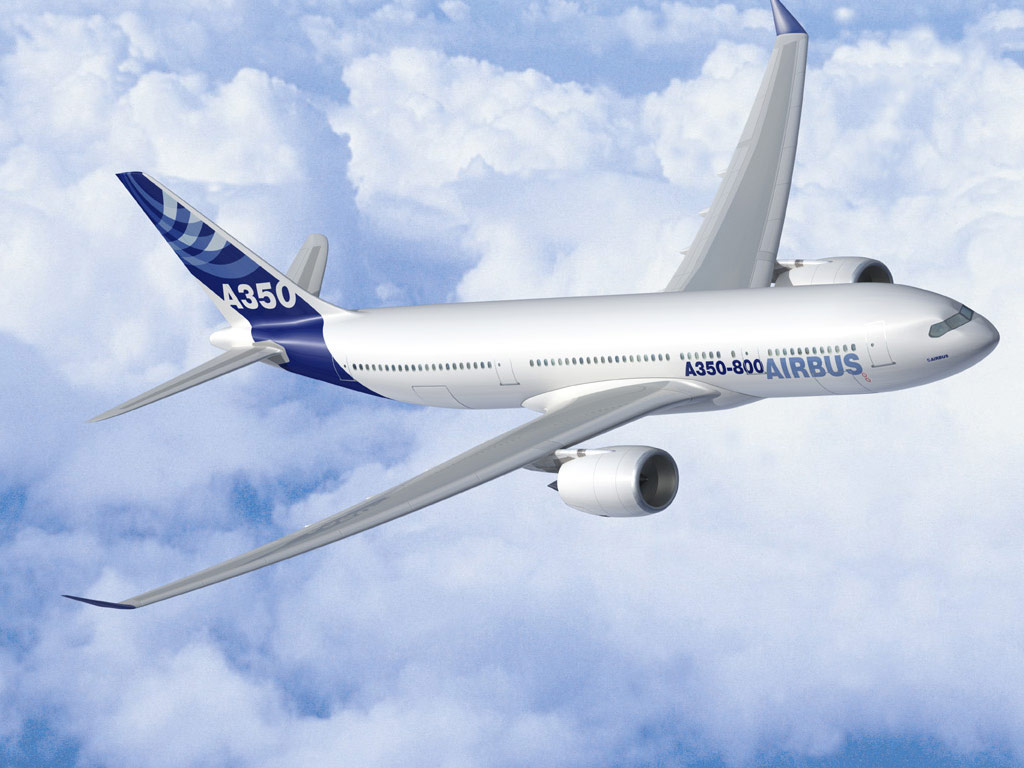
\includegraphics[height=50mm]{Figures/Airbus_A350.jpg}

% Title, author and degree
\vspace{1.0cm}
{\FontLb Thesis Title} \\ % <<<<< EDIT TITLE
%\vspace{0.2cm}
%{\FontMn Subtitle (optional)} \\
%\vspace{1.9cm}
\vspace{2.6cm}
{\FontMb Candidate Full Name} \\ % <<<<< EDIT NAME
\vspace{2.0cm}
{\FontSn \coverThesis} \\
\vspace{0.3cm}
{\FontLb Aerospace Engineering} \\ % <<<<< EDIT COURSE
\vspace{1.0cm}
{\FontSn %
\begin{tabular}{ll}
 \coverSupervisors: & Prof. Full Name 1 \\ % <<<<< EDIT NAME
                    & Dr. Full Name 2    % <<<<< EDIT NAME
\end{tabular} } \\
\vspace{1.0cm}
{\FontMb \coverExaminationCommittee} \\
\vspace{0.3cm}
{\FontSn %
\begin{tabular}{c}
\coverChairperson:     Prof. Full Name          \\ % <<<<< EDIT NAME
\coverSupervisor:      Prof. Full Name 1 (or 2) \\ % <<<<< EDIT NAME
\coverMemberCommittee: Prof. Full Name 3           % <<<<< EDIT NAME
\end{tabular} } \\
\vspace{1.5cm}
{\FontMb Month Year} \\ % <<<<< EDIT DATE (corresponds to date of oral examination)
%
\end{center}

 % file "Thesis_FrontCover.tex"
\cleardoublepage 

% ----------------------------------------------------------------------
% Dedication page (optional)
% ----------------------------------------------------------------------
%%%%%%%%%%%%%%%%%%%%%%%%%%%%%%%%%%%%%%%%%%%%%%%%%%%%%%%%%%%%%%%%%%%%%%%%
%                                                                      %
%     File: Thesis_Dedication.tex                                      %
%     Tex Master: Thesis.tex                                           %
%                                                                      %
%     Author: Andre C. Marta                                           %
%     Last modified :  2 Jul 2015                                      %
%                                                                      %
%%%%%%%%%%%%%%%%%%%%%%%%%%%%%%%%%%%%%%%%%%%%%%%%%%%%%%%%%%%%%%%%%%%%%%%%

\null\vskip5cm%
\begin{flushright}
     Dedicated to my grandmother, Svitlana Sokolovska. Thank you for being beside me and supporting me throughout my life.
\end{flushright}
\vfill\newpage

 % file "Thesis_Dedication.tex"
\cleardoublepage

% ----------------------------------------------------------------------
%  Acknowledgments (optional)
% ----------------------------------------------------------------------
%%%%%%%%%%%%%%%%%%%%%%%%%%%%%%%%%%%%%%%%%%%%%%%%%%%%%%%%%%%%%%%%%%%%%%%%
%                                                                      %
%     File: Thesis_Acknowledgments.tex                                 %
%     Tex Master: Thesis.tex                                           %
%                                                                      %
%     Author: Andre C. Marta                                           %
%     Last modified :  2 Jul 2015                                      %
%                                                                      %
%%%%%%%%%%%%%%%%%%%%%%%%%%%%%%%%%%%%%%%%%%%%%%%%%%%%%%%%%%%%%%%%%%%%%%%%

\section*{\acknowledgments}

% Add entry in the table of contents as section
\addcontentsline{toc}{section}{\acknowledgments}

A few words about the university, financial support, research advisor, dissertation readers, faculty or other professors, lab mates, other friends and family...

 % file "Thesis_Acknowledgements.tex"
\cleardoublepage

% ----------------------------------------------------------------------
%  Abstract (both in English and Portuguese)
% ----------------------------------------------------------------------
%%%%%%%%%%%%%%%%%%%%%%%%%%%%%%%%%%%%%%%%%%%%%%%%%%%%%%%%%%%%%%%%%%%%%%%%
%                                                                      %
%     File: Thesis_Resumo.tex                                          %
%     Tex Master: Thesis.tex                                           %
%                                                                      %
%     Author: Andre C. Marta                                           %
%     Last modified :  2 Jul 2015                                      %
%                                                                      %
%%%%%%%%%%%%%%%%%%%%%%%%%%%%%%%%%%%%%%%%%%%%%%%%%%%%%%%%%%%%%%%%%%%%%%%%

\section*{Resumo}

% Add entry in the table of contents as section
\addcontentsline{toc}{section}{Resumo}

Inserir o resumo em Portugu\^{e}s aqui com o máximo de 250 palavras e acompanhado de 4 a 6 palavras-chave...

\vfill

\textbf{\Large Palavras-chave:} palavra-chave1, palavra-chave2,...

   % file "Thesis_Resumo.tex"
\cleardoublepage

%%%%%%%%%%%%%%%%%%%%%%%%%%%%%%%%%%%%%%%%%%%%%%%%%%%%%%%%%%%%%%%%%%%%%%%%
%                                                                      %
%     File: Thesis_Abstract.tex                                        %
%     Tex Master: Thesis.tex                                           %
%                                                                      %
%     Author: Andre C. Marta                                           %
%     Last modified :  2 Jul 2015                                      %
%                                                                      %
%%%%%%%%%%%%%%%%%%%%%%%%%%%%%%%%%%%%%%%%%%%%%%%%%%%%%%%%%%%%%%%%%%%%%%%%

\section*{Abstract}

% Add entry in the table of contents as section
\addcontentsline{toc}{section}{Abstract}

\gls{tls} is one of the most used communication security protocols in the world. It comes with many configurations. 
Each configuration offers a set o security services, which has an implication on the 
security level and computational cost.
Not all of those configurations can be used with the resource constrained \gls{iot} devices, due to the
high computational and memory demands. Most of the existing work focuses on \gls{dtls}
and cannot be easily integrated with existing deployments. Existing work fails
to evaluate the cost of various \gls{tls} configurations and its security services.
This work focuses on cost analysis of the security services of the TLS protocol.
We evaluate the number of CPU cycles used and time taken by each \gls{tls} configuration
and security service. Software developers can use this information
to make security/cost trade-offs based on the environment needs and limitations.  

\vfill

\textbf{\Large Keywords:} TLS, DTLS, SSL, IoT, embedded systems

 % file "Thesis_Abstract.tex"
\cleardoublepage

% ----------------------------------------------------------------------
%  Table of contents, list of tables, list of figures and nomenclature
% ----------------------------------------------------------------------

% Table of contents
%
\tableofcontents
\cleardoublepage 

% List of tables
%
% Add entry in the table of contents as section
\phantomsection
\addcontentsline{toc}{section}{\listtablename}
% Generate list
\listoftables
\cleardoublepage 

% List of figures
%
% Add entry in the table of contents as section
\phantomsection
\addcontentsline{toc}{section}{\listfigurename}
% Generate list
\listoffigures
\cleardoublepage 

% Nomenclature
%
% entries of nomenclature list
%%%%%%%%%%%%%%%%%%%%%%%%%%%%%%%%%%%%%%%%%%%%%%%%%%%%%%%%%%%%%%%%%%%%%%%%
%                                                                      %
%     File: Thesis_Nomenclature.tex                                    %
%     Tex Master: Thesis.tex                                           %
%                                                                      %
%     Author: Andre C. Marta                                           %
%     Last modified : 21 Jan 2011                                      %
%                                                                      %
%%%%%%%%%%%%%%%%%%%%%%%%%%%%%%%%%%%%%%%%%%%%%%%%%%%%%%%%%%%%%%%%%%%%%%%%
%
% The definitions can be placed anywhere in the document body
% and their order is sorted by <symbol> automatically when
% calling makeindex in the makefile
%
% The \glossary command has the following syntax:
%
% \glossary{entry}
%
% The \nomenclature command has the following syntax:
%
% \nomenclature[<prefix>]{<symbol>}{<description>}
%
% where <prefix> is used for fine tuning the sort order,
% <symbol> is the symbol to be described, and <description> is
% the actual description.

% ----------------------------------------------------------------------
% Roman symbols [r]
\nomenclature[ru]{$\bf u$}{Velocity vector.}
\nomenclature[ru]{$u,v,w$}{Velocity Cartesian components.}
\nomenclature[rp]{$p$}{Pressure.}
\nomenclature[rC]{$C_D$}{Coefficient of drag.}
\nomenclature[rC]{$C_L$}{Coefficient of lift.}
\nomenclature[rC]{$C_M$}{Coefficient of moment.}

% ----------------------------------------------------------------------
% Greek symbols [g]
\nomenclature[g]{$\rho$}{Density.}
\nomenclature[g]{$\alpha$}{Angle of attack.}
\nomenclature[g]{$\beta$}{Angle of side-slip.}
\nomenclature[g]{$\mu$}{Molecular viscosity coefficient.}
\nomenclature[g]{$\kappa$}{Thermal conductivity coefficient.}

% ----------------------------------------------------------------------
% Subscripts [s]
\nomenclature[s]{$x,y,z$}{Cartesian components.}
\nomenclature[s]{$i,j,k$}{Computational indexes.}
\nomenclature[s]{$\infty$}{Free-stream condition.}
\nomenclature[s]{ref}{Reference condition.}
\nomenclature[s]{$n$}{Normal component.}

% ----------------------------------------------------------------------
% Supercripts [t]
\nomenclature[t]{T}{Transpose.}
\nomenclature[t]{*}{Adjoint.}

 % file "Thesis_Nomenclature.tex"
%
% Add entry in the table of contents as section
\phantomsection
\addcontentsline{toc}{section}{\nomname}
% Insert glossary/nomenclature section produced by MakeIndex
\printnomenclature
\cleardoublepage

% entries of glossary list
%%%%%%%%%%%%%%%%%%%%%%%%%%%%%%%%%%%%%%%%%%%%%%%%%%%%%%%%%%%%%%%%%%%%%%%%%
%                                                                      %
%     File: Thesis_Glossary.tex                                        %
%     Tex Master: Thesis.tex                                           %
%                                                                      %
%     Author: Andre C. Marta                                           %
%     Last modified : 30 Oct 2012                                      %
%                                                                      %
%%%%%%%%%%%%%%%%%%%%%%%%%%%%%%%%%%%%%%%%%%%%%%%%%%%%%%%%%%%%%%%%%%%%%%%%
%
% The definitions can be placed anywhere in the document body
% and their order is sorted by <symbol> automatically when
% calling makeindex in the makefile
%
% The \glossary command has the following syntax:
%
% \glossary{entry}
%
% The \nomenclature command has the following syntax:
%
% \nomenclature[<prefix>]{<symbol>}{<description>}
%
% where <prefix> is used for fine tuning the sort order,
% <symbol> is the symbol to be described, and <description> is
% the actual description.

% ----------------------------------------------------------------------

\glossary{name={\textbf{MDO}},description={Multi-Disciplinar Optimization is an engineering technique that uses optimization methods to solve design problems incorporating two or more disciplines.}}

\glossary{name={\textbf{CFD}},description={Computational Fluid Dynamics is a branch of fluid mechanics that uses numerical methods and algorithms to solve problems that involve fluid flows.}}

\glossary{name={\textbf{CSM}},description={Computational Structural Mechanics is a branch of structure mechanics that uses numerical methods and algorithms to perform the analysis of structures and its components.}}



 % file "Thesis_Glossary.tex"

% Add entry in the table of contents as section
%\phantomsection
%\addcontentsline{toc}{section}{\glossaryname}
% Insert glossary section produced by MakeIndex
%\cleardoublepage

% Set arabic numbering (1,2,...) after preface
%
\setcounter{page}{1}
\pagenumbering{arabic}

% ----------------------------------------------------------------------
%  Chapters
% ----------------------------------------------------------------------

%%%%%%%%%%%%%%%%%%%%%%%%%%%%%%%%%%%%%%%%%%%%%%%%%%%%%%%%%%%%%%%%%%%%%%%%
%                                                                      %
%     File: Thesis_Introduction.tex                                    %
%     Tex Master: Thesis.tex                                           %
%                                                                      %
%     Author: Andre C. Marta                                           %
%     Last modified :  2 Jul 2015                                      %
%                                                                      %
%%%%%%%%%%%%%%%%%%%%%%%%%%%%%%%%%%%%%%%%%%%%%%%%%%%%%%%%%%%%%%%%%%%%%%%%

\chapter{Introduction}
\label{chapter:introduction}

In recent years there has been a sharp increase in the number of \gls{iot}
devices and this trend is expected to continue\cite{IoTnumb83:online}. The IoT is a network
of interconnected devices, which exchange data with one another over
the internet. In fact, it can be any object that has an assigned
IP address and is provided with the ability to transfer data over a network. 
While there are many types of IoT devices, all of them
are restricted: they have limited memory, processing power and
available energy. Examples of IoT devices include temperature sensors,
smart light bulbs and physical activity trackers.
Even a salt shaker\cite{SMALTThe76:online} can now be part of the global network.

The \gls{iot} technology provides many benefits, from personal comfort to
transforming entire industries, mainly due to increased connectivity and
new sources for data analysis. The technological development, however, tends to focus on
innovative design rather than on security. \gls{iot} devices frequently
connect to networks using inadequate security and are hard to update when
vulnerabilities are found.

This lack of security in the \gls{iot} ecosystem has been exploited by the
the \textit{Mirai} botnet\cite{sec17ant94:online} when it overwhelmed several high-profile
targets with massive \gls{ddos} attacks. This is the most devastating attack involving \gls{iot}
devices done to date. However, the \textit{Reaper} botnet\cite{ReaperCa10:online} could be
even worse if it is ever put to malicious use. Similar attacks will inadvertently
come in the future.

In the process of the work on this dissertation, we have made several
contributions to the \gls{tls} $1.3$ specification, and were formally recognized as 
contributors\cite{Mergepul65:online}. Our name can be found in the document specifying \gls{tls} $1.3$\cite{RFC8446}.
Although to the lesser extent, we have also contributed to \gls{dtls} $1.3$ specification\cite{DTLS13:online}.
We have found a security issue within the
\gls{tls} implementation of the \textit{mbedTLS} library. We reported it and it
has been assigned a \textit{CVE} with the id \textit{CVE-2018-1000520}\cite{NVDCVE2094:online}.
It is an authentication problem, where certificates signed with an incorrect algorithm
were accepted in some cases. More specifically, \textit{ECDH(E)-RSA} ciphersuites allowed \gls{ecdsa}-signed
certificates, when only \gls{rsa}-signed ones should have been. We also found a bug in \textit{mbedTLS}'s test suite
related to the use of deprecated \textit{SHA-1}-signed certificates and submitted a code fix to 
it\cite{sslserve89:onelin}\cite{updatete23:online}.

\section{Motivation}
%

While inter-device communication has numerous benefits, it is important
to ensure the security of that communication. For example, when you log
in to your online banking account, you do not want others to be
able to see your password, as this may lead to the compromise of your
account. Having your account compromised means that a malicious entity
might steal your money. Similarly, when you are transferring funds via
online banking, you want the contents of that operation to be
invisible to an observer, for privacy reasons. It is also desirable
that no party is able to tamper with the data en transit,
as it may lead to undesired consequences, such as the transfer of a
larger amount than intended. Proper communication security allows
those goals to be achieved.

\gls{tls} is one of the most used protocols for communication security. It
powers numerous technologies, such as \gls{https}. TLS offers the
security services of authentication, confidentiality, privacy, integrity, replay
protection and perfect forward secrecy. It is not a requirement to use all of
those services for every TLS connection. The protocol is similar to
a framework, in the sense that you can enable individual security
services on a per-connection basis. For example, when you are downloading
software updates, while data confidentiality is probably not a concern,
data authenticity and integrity, are. In \gls{tls}, it is possible for a connection
to only offer authenticity and integrity, without offering confidentiality.
Foregoing unnecessary services will lead to a smaller resource usage,
which in turn leads to smaller execution time and power usage. This
is especially important in the context of IoT, due to the constrained
nature of the devices. 

Existing work does not explore the computational costs
of the security services available in \gls{tls}. Examples of such costs are the 
number of CPU cycles executed, time taken and power used.  
Thus, developers wishing to deploy the \gls{tls} protocol
in constrained environments do not have a resource that would help them in choosing a \gls{tls}
configuration appropriate to the environment's needs and limitations.

\gls{tls} is designed to run on top of a reliable, connection-oriented
protocol, such as TCP. \gls{dtls} is the version of \gls{tls} that runs on top
of an unreliable transport protocol, such as UDP. Most \gls{iot} devices have
very limited processing power, storage and energy. Moreover, the performance of
TCP is known to be inefficient in wireless networks, due to its congestion control
algorithm. This situation is worsened with the use of low-power radios and lossy
links found in sensor networks. Therefore, in many cases the use of TCP with \gls{iot}
is not the best option. For this reason, \gls{dtls}, which runs on top
of UDP, is used more frequently in such devices. 
While the work of this dissertation will be focused on \gls{tls}, the majority of it
can also be applied to \gls{dtls}. This is a consequence of \gls{dtls} being 
just an adaption of \gls{tls} over unreliable  transport protocols, 
without changes to the core protocol.

There are numerous IoT devices, each one with different hardware
capabilities and security requirements. For example, some IoT
devices have the resources to use public key cryptography,
while for others symmetric cryptography is the only option.
In some cases, the communicating devices require data authenticity, confidentiality
and integrity (e.g. when logging in into a device), while in others data
authenticity and integrity is enough (e.g. when transferring updates).

\gls{tls} was not designed for the constrained environment of IoT. Despite that,
it is a malleable protocol and can be configured to one's needs. In essence,
it is a combination of various security algorithms that together form
a protocol for communication security. If configured
properly, it is possible to use it in the context of IoT.

The majority of existing work on \gls{tlsd} optimization proposes 
a solution that is either tied to a
specific protocol, such as \gls{coap}, or requires an introduction of a third-party
entity, such as the trust anchor in the case of the S3K system\cite{S3KScala62:online} or
even both. This has two main issues. First, a protocol-specific solution cannot
be easily used in an environment where (D)\gls{tls} is not used with that protocol.
Second, the requirement of a third-party
introduces additional cost and complexity, which will be a big resistance factor
in adopting the technology. This is especially true for developers working on
personal projects or projects for small businesses, leaving the communications insecure
in the worse case scenario. Therefore a solution that is protocol independent and fully 
compatible with the \gls{tlsd} standard and existing infrastructure is desired.

Another issue with the existing literature is that it almost exclusively focuses on \gls{dtls} optimization
and not all of it can be applied to \gls{tls}. Herein we want to further explore \gls{tls} optimization. 
There is clearly a need for that,
especially with \gls{coap} over TCP and \gls{tls} standard\cite{I-D.ietf-core-coap-tcp-tls} being currently developed. The
mentioned standard does not explore any \gls{tls} optimizations, and since any
\gls{iot} device using it in the future would benefit from them, this is an important
area to explore.

\section{Objectives}

(D)\gls{tls} is a complex protocol with numerous possible configurations. Each configuration
provides different set security services and a different security level. This has a direct
impact on the resource usage. Thus, the cost of a \gls{tlsd} connection can be lowered,
by using an appropriate configuration. Typically, this involves making security/cost trade-offs.
Optimizing the connection cost by selecting one of the numerous configurations available in \gls{tlsd}
 meets our goals of being protocol independent, fully compatible with
existing infrastructure and targeting \gls{tls} optimization specifically.

The objective of this work is to provide a means of assisting application developers
who wish to include secure communications in their applications to make
security/resource usage trade-offs, according to the environment's needs
and limitations. We will give a general overview of of the costs of the \gls{tls} protocol as a whole and
of its individual parts. This is will allow us to answer questions such as \textit{How much will we save if we use protocol X instead of Y for authentication?}.
Thus, performing evaluations on specific \gls{iot} hardware or analyzing \gls{tls}-specific optimizations
on it is outside of the scope of this paper.

In order to achieve our goal, the cost of each individual security service
will be evaluated. With this information, the programer will be able to choose a configuration that
meets his security requirements and device constraints. If the limitations of the device's hardware
do not allow to meet the requirements, the programer may decide on an alternative configuration, possibly with
a loss of some security services and a lower security level, or forgo using (D)\gls{tls} altogether.
Thus, this work is targeted towards developers and InfoSec professionals who wish to add communication security
to applications in the IoT environment.

In our work, we evaluated the \textit{mbedTLS 2.7.0}'s\cite{SSLLibra13:online} implementation of the \gls{tls} protocol version $1.2$.
\textit{mbedTLS} is among the most popular libraries with a \gls{tls} implementation for embedded systems. \gls{tls} protocol 
version $1.2$ is currently the most used version of \gls{tls} on the internet \cite{QualysSS90:online}. The work on
the dissertation started before \gls{tls} protocol's version $1.3$ specification was finished and there were no embedded device
libraries which implemented it.  For this reason we did not evaluate \gls{tls} $1.3$. Despite that, the results
obtained in this work apply to it as well, since the core functionality of the security services remained mostly unchanged.

We used two cost metrics: the estimated number of CPU cycles and the time taken. The time values were read direcly from
the processor's registers. The profiled instructions are CPU-bound, thus the number of CPU cycles will be proportional to time,
as will later show in our analysis. Later in the text we will show that our esitmates do reflect real values, by comparing them to time
measurments obtained directly from the CPU registers. Section \ref{sec:eval-metrics-and-lims} contains a detailed description of the 
evaluated costs and their limitations.

\section{Results}

In summary, the results of this work are enumerated as follows:

\begin{enumerate}
  \item Evaluate the costs of the security services of confidentiality, integrity, \gls{pfs} and authentication in \gls{tls}
  \item Evaluate and compare the costs of various alternative algorithms which can be used to provide each one of the security services
  \item Evaluate and compare the costs of all of the possible \gls{tls} configurations present in \textit{mbedTLS 2.7.0}
  \item Contribute to the \gls{tls} protocol's version $1.3$ specification
  \item Contribute to the \gls{dtls} protocol's version $1.3$ specification
  \item Find and report a security vulnerability present in \textit{mbedTLS 2.7.0}
  \item Find, report and submit a patch to fix a bug present in \textit{mbedTLS 2.7.0}
\end{enumerate}

\section{Structure of The Document}

The document is organized as follows: Section 2 describes the background. It
introduces some of the concepts that will be used throughout
the document. Section 3 describes the \gls{tls} and \gls{dtls} protocol
versions $1.2$ and $1.3$, with a focus on the version $1.2$ since
it is the latest and the most used version of the protocol at the time we started this work (version $1.3$ was still in
draft mode). Section 4 describes all of the related work done in the area and
the current state of the art. Section 5 describes the objectives of the work and evaluation 
are described in more detail. 
Section 6
covers the evaluation's methodology and limitations. In Section 7 we evaluate the costs of the various \gls{tls}
configurations and their individual parts. Finally, the conclusion of the work is done in Section 8. % file "Thesis_Introduction.tex"
\cleardoublepage

%%%%%%%%%%%%%%%%%%%%%%%%%%%%%%%%%%%%%%%%%%%%%%%%%%%%%%%%%%%%%%%%%%%%%%%%
%                                                                      %
%     File: Thesis_Background.tex                                      %
%     Tex Master: Thesis.tex                                           %
%                                                                      %
%     Author: Andre C. Marta                                           %
%     Last modified :  2 Jul 2015                                      %
%                                                                      %
%%%%%%%%%%%%%%%%%%%%%%%%%%%%%%%%%%%%%%%%%%%%%%%%%%%%%%%%%%%%%%%%%%%%%%%%
\chapter{Background}
\label{chapter:background}

This chapter will begin with a summary of the most relevant theoretical background. This is done is Section \ref{crypto-algs}.
After that, in Section \ref{related-work} we describe the current state of art in the topic of this work.

\section{Cryptograpic Algorithms} \label{crypto-algs}

\gls{tls} is a complex protocol that relies on various cryptographic algorithms to provide
security. The most relevant ones will be described here.

In a typical scenario, \gls{tls} uses \gls{ac} for peer authentication and \gls{sc} for bulk data
encryption and integrity protection, for this reason this topic will be covered in Section \ref{sac}. Section \ref{pccc} covers the most common way of peer authentication: public key certificates. Authenticated Encryption With Additional Data (AEAD) ciphers offer various advantages in the
context of \gls{iot}, particularly less computational and spacial overhead.
Furthermore, they are the only type of ciphers that can be used in \gls{tls}
$1.3$. For those reasons, they're covered in Section \ref{aeadciphers}.
When compared to other public key cryptography approaches, \gls{ecc} offers shorter keys, lower processing requirements and lower memory usage for equivalent security strength, being heavily used
in \gls{tls}. An overview of \gls{ecc} in presented in Section \ref{eccsection}.


\subsection{Symmetric vs Asymmetric Cryptography} \label{sac}

\gls{ac} is more expensive than \gls{sc} in terms of performance. There are two main reasons for this. First, larger key sizes are required for an \gls{ac} system to achieve the
same level of security as in a \gls{sc} system. Second, \textit{CPU}s are slower at performing the underlying
mathematical operations involved in \gls{ac}, namely exponentiation requires
$O(log e)$ multiplications for an exponent $e$. The 2016 \textit{NIST} report \cite{Recommen44:online}
suggests that an \gls{ac} algorithm would need to use a secret key with size of \textit{15360 bits}
to have equivalent security to a \textit{256-bit} secret key for a \gls{sc} algorithm.
This situation is ameliorated by \gls{ecc}, which requires keys of \textit{512 bits}, but
it is still slower than using \gls{sc}. The 2017 \textit{BSI} report \cite{Kryptogr1:online} (from the
German federal office for information security) suggests similar numbers.

Another argument for avoiding the use of \gls{ac}
algorithms as much as possible, is that they require additional storage space. This can be a problem for many \gls{iot} devices,
like \textit{class 1} devices according to the terminology of constrained-code
networks\cite{RFC7228} which have approximately \textit{10KB} of RAM and \textit{100KB}
of persistent memory. We measured and compared the resulting size of the \textit{mbedTLS 2.7.0} library\cite{SSLLibra13:online} binary when it was compiled with and without the \gls{rsa} module
(located in the \textit{rsa.c} file). The conclusion is that that using the \textit{rsa.c} module adds an overhead of about \textit{32KB}.

\subsection{Public Certificates and Certificate Chains} \label{pccc}

A public key certificate, also known as a digital certificate, is an electronic
document used to prove the ownership of a public key. This allows other parties
to rely upon assertions made by the private key that corresponds to the public key
that is certified. In the context of (D)\gls{tls}, certificates serve as a guarantee
that the communication is done with the claimed entity and not someone impersonating it.

A \gls{ca} is an entity that issues digital certificates. There are two types of
\gls{ca}s: the \textbf{root \gls{ca}s} and the \textbf{intermediate \gls{ca}s}.
An intermediate \gls{ca} is provided with a certificate with signing capabilities
signed by one of the root \gls{ca}s. A \textbf{certificate chain} is a list of
certificates from the root certificate to the end-user certificate, including
any intermediate certificates along the way. In order for a certificate
to be trusted by a device, it must be directly or indirectly issued by a \gls{ca} trusted by the device.

In (D)\gls{tls}, the certificates are in the \textit{X.509} format, defined
in \textit{RFC 5280}\cite{rfc5280}.

\subsection{\gls{aead} Ciphers} \label{aeadciphers}

\gls{ae} and \gls{aead} are forms of encryption which simultaneously provide
confidentiality, integrity and authenticity guarantees on the data. An \gls{ae}
cipher takes as input a \textit{key}, a \textit{nonce} and a \textit{plaintext}
and outputs the pair \textit{(ciphertext, MAC)}, if it is encrypting and does the inverse
process, while also performing the \gls{mac} check if it is decrypting.

\gls{aead} is nothing more than a variant of \gls{ae}, which comes with an extra
input parameter that is additional data, that is \textbf{only authenticated, but not encrypted}.
Some \gls{aead} ciphers have shorter authentication tags (\textit{i.e.} shorter \gls{mac}s),
which makes then more suitable for low-bandwidth networks, since the messages to be sent are smaller in size.

\subsection{\gls{ecc}} \label{eccsection}

Public key cryptography is based on the use of one-way math functions. Such
functions make it easy to compute the answer given an input,
but hard to compute the input given the answer. For example, RSA uses factoring
as the one one way function: it is easy to multiply large numbers, but it is hard
to factor them.

\gls{ecc} is based on elliptic curves, which are set of points $(x,y)$ that are
solutions to the equation $y^2 = x^3 + ax + b$, where $4a^3 + 27b^2 \neq 0$.
Depending on the value of $a$ and $b$, elliptic curves assume different shapes
on the plane.

The security of \gls{ecc} is based on the elliptic curve discrete logarithm
problem. It states that scalar multiplication is a one way function. To exemplify,
given a curve $E(\mathbb{Z}/p\mathbb{Z})$ and points $Q$ and $P$ on that curve
$Q,P \in E(\mathbb{Z}/p\mathbb{Z})$, where $Q$ is a multiple of $P$, the elliptic curve discrete logarithm problem
states that finding the integer $k$, such that $Q=kP$ is a very hard problem.

\section{The \gls{tls} Protocol}

\gls{tls} is a \textbf{client-server} protocol
that runs on top a \textbf{connection-oriented and reliable transport protocol},
such as \textbf{TCP}. Its main goal is to provide \textbf{privacy} and \textbf{integrity}
between the two communicating peers. Privacy implies that a third party will not
be able to read the data, while integrity means that a third party will not be
able to alter the data.

In the TCP/IP Protocol Stack, \gls{tls} is placed between the \textbf{Transport}
and \textbf{Application} layers. It is designed to simplify the establishment
and use of secure communications from the application developer's standpoint.
The developer's task is reduced to creating a "secure" connection (\textit{i.e.} socket), instead of a "normal" one.

A secure communication established using \gls{tls} has two phases. In the first
phase, the communicating peers authenticate one to another and negotiate the parameters, such as the secret keys and the encryption algorithm. In the
second phase, they exchange cryptographically protected data under
the previously negotiated parameters. The first phase is done under the
Handshake Protocol and the second under the Record Protocol. In order to
achieve its goals, during the Handshake Protocol the client and the server
exchange various messages. The message flow is depicted in Figure \ref{fig:tls-12-handshake} and described in more detail in Section
\ref{hsp}.

\gls{tls} provides the following \textbf{security services}:
\begin{itemize}
\item \textbf{authentication} - both, \textbf{peer entity} and \textbf{data origin} (or \textbf{integrity})
authentication.
\subitem \textbf{peer entity authentication} - a peer has a guarantee that it is talking to certain entity, for example, \textit{www.google.com}.
This is achieved thought the use of \gls{ac}, also known as \gls{pkc}, (\textit{e.g.} \textit{RSA} and \textit{DSA})
or \textbf{symmetric key cryptography}, using a \gls{psk}.
\item \textbf{confidentiality} - the data transmitted between the communicating
entities (the client and the server) is encrypted. Symmetric cryptography is
used for data encryption (\textit{e.g.}, \textit{AES}).
\item \textbf{integrity} (also called \textbf{data origin authentication}) - a peer can be sure that the data was not modified or forged,
\textit{i.e.}, there is a guarantee that the received data is coming from the expected entity. For example, a peer can be sure
that the \textit{index.html} file that was sent to when it connected to \textit{www.google.com} did, in fact,
come from \textit{www.google.com} and it was not tampered with by an attacker (\textbf{data integrity}). This is achieved either through the use
of a keyed \gls{mac} or an \gls{aead} cipher.
\item \textbf{replay protection} (also known as \textbf{freshness}) -
a peer can be sure that a message has not been replayed. This is
achieved through the use of sequence numbers. Each \gls{tls} record has a different sequence number, which is incremented. If a non-\gls{aead} cipher is used, the sequence number is a direct input of the \gls{mac} function. If an \gls{aead} cipher is used, a nonce derived from the sequence number is used as input to that cipher.
\end{itemize}

Despite using \gls{pkc}, \gls{tls} does \textbf{not} provide \textbf{non-repudiation services}:
neither \textbf{non-repudiation with proof of origin}, which addresses the peer denying
the sending of a message, nor \textbf{non-repudiation with proof of delivery}, which
addresses the peer denying the receipt of a message. This is due to the fact that
instead of using \textbf{digital signatures}, either a keyed \gls{mac} or an \gls{aead}
cipher is used, both of which require a secret to be \textbf{shared} between the peers.

It is not required to use all of the tree security services every situation.
In this sense, \gls{tls} is like a framework that allows to select which security services should be used for a communication session. As an example,
certificate validation might be skipped, which means that the \textbf{authentication} guarantee is not provided. There are some differences regarding this claim between \gls{tls} $1.2$\cite{RFC5246}
and \gls{tls} $1.3$. For example, while in the first there is a \textit{null}
cipher (no authentication, no confidentiality, no integrity), in the latter
this is not true, since it deprecated all non-\gls{aead} ciphers in favor of
\gls{aead} ones.

The terms \gls{ssl} and \gls{tls} are often used interchangeably, but one is
a predecessor of another - \gls{ssl} $3.0$\cite{RFC6101} served as the basis
for \gls{tls} $1.0$\cite{RFC6101}.

Section \ref{subprotocols} will begin with a brief overview of the various sub-protocols that compose \gls{tls}. The \gls{tls} Record Layer will
be described in sufficient detail for the \gls{tls} Handshake Protocol
description that follows in Section \ref{hsp}. The way each record is
processed when sending and receiving data is covered in Section \ref{record}.
The symmetric keys involved in cryptographic operations that provide
confidentiality and security are described in Section \ref{keying}. Section
\ref{keying-material} explains how those keys are generated in \gls{tls} 1.2.
There are various methods that the client and the server can use to exchange
keys, those will be covered in Section \ref{key-exchange}. The \gls{tls}
Extension mechanism will be covered in Section \ref{extensions}. There
are various differences from \gls{tls} $1.2$ to $1.3$ and those that were
not covered in the previous sections will be in Section \ref{tls-13}.
This section ends with an outline of the main differences from \gls{dtls} to \gls{tls} in Section \ref{dtls}.


\subsection{\gls{tls} (Sub)Protocols} \label{subprotocols}

\gls{tls} is composed of several protocols, which are illustrated in Figure
\ref{fig:tls-subprotocols} and briefly described below:
\begin{itemize}
  \item \textbf{\gls{tls} Record Protocol} - the lowest layer in \gls{tls}.
  It takes messages to be transmitted, fragments the data into manageable
  blocks, optionally compresses them, encrypts them and transmits the result.
  When the data is received, the reverse process is done. The \gls{tls}
  Record Protocol is located directly on top of \textbf{TCP/IP} and it serves as an
   \textbf{encapsulation for the remaining sub-protocols} (\textit{4} in case of \gls{tls} 1.2
   and \textit{3} in case of \gls{tls} 1.3). To the  \textbf{Record Protocol},
   the remaining sub-protocols are what \textit{TCP/IP} is to \textit{HTTP}.
   A \gls{tls} Record is comprised of 4 fields, with the first 3 comprising the
   \gls{tls} Record header. The first field is a 1-byte record \textit{type}
   specifying the type of record that is encapsulated (ex: value \textit{0x16}
   for the handshake protocol). The second is a 2-byte \textit{TLS version} field. The third is a
   2-byte \textit{length} field specifying the length of the data in the record, excluding
   the header itself (this means that \gls{tls} has a maximum record size
   of \textit{16384} bytes). The fourth is a \textit{fragment} field,
   containing \textit{length} bytes of data that is
   transparent to the Record layer and should be dealt by a higher-level protocol. That higher-level protocol is specified by the \textit{type} field. This is illustrated in Figure \ref{fig:tls-record-header}.
  \item \textbf{\gls{tls} Handshake Protocol} - the core protocol of \gls{tls}.
  It allows the communicating peers to \textbf{authenticate} one to another and to negotiate the connection state. In \gls{tls} 1.2
  a \textbf{cipher suite} and a \textbf{compression} method are negotiated. In \gls{tls} $1.3$, a \textbf{cipher suite} and a \textbf{key exchange} algorithm are negotiated. The agreed upon \textbf{cipher suite} is used to provide the previously described security services. In
  \gls{tls} $1.2$, a \textbf{cipher suite} consists of a \textbf{cipher spec},
  a \textbf{key exchange} algorithm and a \gls{prf}, which is used for key generation.
  In \gls{tls} $1.2$,
  \textbf{cipher spec} defines the message encryption algorithm and the message
  authentication algorithm. In \gls{tls} 1.3, the term
   \textbf{cipher spec} is no longer present, since the \textbf{ChangeCipherSpec}
   protocol has been removed. The concept of \textbf{cipher suite} has been updated
   to define the pair consisting of an \gls{aead} algorithm and a hash function to be used with
   \gls{hkdf}. In \gls{tls} $1.3$ the \textbf{key exchange} algorithm is negotiated via
   extensions.
  \item \textbf{\gls{tls} Alert Protocol} - allows the communicating peers to
  signal potential problems.
  \item \textbf{\gls{tls} Application Data Protocol} - used to transmit application data messages securely using the security parameters negotiated during the \textbf{Handshake Protocol}. The messages are treated as transparent data to the record layer.
  \item \textbf{\gls{tls} Change Cipher Spec Protocol} (removed in \gls{tls} 1.3) -
  used to activate the initial \textbf{cipher spec} or change it during the connection.
\end{itemize}

% src: https://tex.stackexchange.com/questions/5769/two-figures-side-by-side

\begin{figure}
  \centering
  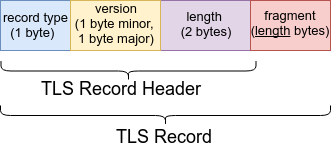
\includegraphics[width=0.6\textwidth]{img/record-header-3.png} % first figure itself
  \caption{\label{fig:tls-record-header} TLS Record header}
\end{figure}

\begin{figure}
\centering
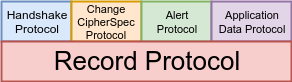
\includegraphics[width=0.6\textwidth]{img/tls-sub-protocols-3.png} % second figure itself
\caption{\label{fig:tls-subprotocols} TLS (Sub)protocols and Layers}
\end{figure}

\subsection{TLS 1.2 Handshake Protocol} \label{hsp}

The Handshake Protocol is responsible for negotiating a \textbf{session},
which will then be used in a \textbf{connection}.
There is a difference between a \gls{tls} session and a \gls{tls} connection:
\begin{itemize}
  \item \textbf{TLS session} - association between two communication peers that is
  created by the \textbf{TLS Handshake Protocol}, which defines a set of negotiated parameters
  (cryptographic and others, such as
  the compression algorithm, depending on the \gls{tls} version) that are used by the \textbf{TLS connections associated
  with that session}. A single \textbf{TLS session} can be shared among multiple
  \textbf{TLS connections} and its main purpose is to avoid the expensive negotiation
  of new parameters for each \textbf{TLS connection}. For example, let us say
  that a \gls{html} page is being downloaded over the \gls{https} and that page references some images from that same server using \gls{https} links. Instead of the web browser negotiating a new \gls{tls} session for every single image again, it can re-use the the
  one it has established to download the \gls{html} page,
  saving time and computational resources. Session resumption can be done using various
  approaches, such as \textbf{session identifiers}, described throughout \textit{Section 7.4}
  of \textit{RFC 5246}\cite{RFC5246} and \textbf{session tickets}, defined in
  \textit{RFC 5077}\cite{RFC5077}.
  \item \textbf{TLS connection} - used to actually transmit the cryptographically
  protected data. For the data to be cryptographically protected, some parameters,
  such as the secret keys used to encrypt and authenticate the transmitted
  data need to be established; this is done when a \textbf{TLS session} is created,
  during the \textbf{TLS Handshake Protocol}.
\end{itemize}

\begin{figure}
        \centering
        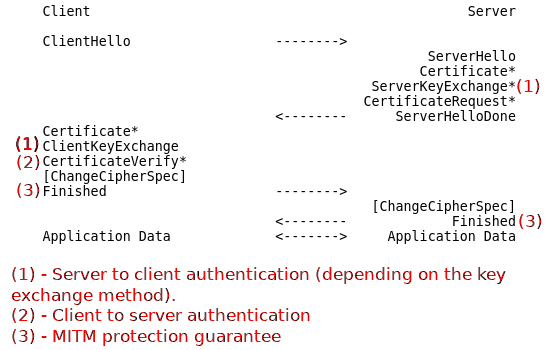
\includegraphics[width=0.9\textwidth]{img/tls-12-full-handshake2.png} % first figure itself
        \caption{\label{fig:tls-12-handshake} \gls{tls} $1.2$ message flow for a full handshake}
\end{figure}

\begin{figure}
  \centering
  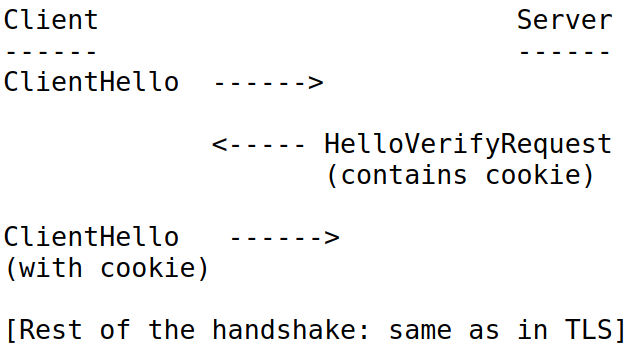
\includegraphics[width=0.6\textwidth]{img/dtls-cookie.png} % second figure itself
  \caption{\label{fig:dtls-cookie} DTLS handshake with HelloVerifyRequest containing the cookie}
\end{figure}


In the handshake phase the client and the server agree on which version of the \gls{tls}
protocol to use, authenticate one to another and negotiate session state items like
the cipher suite and the compression method.  Figure \ref{fig:tls-12-handshake} shows the message flow for the
full \gls{tls} $1.2$ handshake. \textit{*} indicates situation-dependent
messages that are not always sent. \textit{ChangeCipherSpec} is a separate
protocol, rather than a message type.

As already mentioned, every \gls{tls} handshake message is encapsulated within
a \gls{tls} record. The actual handshake message is contained within the
\textit{fragment} of a \gls{tls} record. The record type for a handshake
message is \textit{0x16}. The handshake message has the following structure:
a 1-byte \textit{msg\_type} field (specifies the Handshake message type),
a 2-byte \textit{length} field (specifies the length of the \textit{body})
and a \textit{body} field, which contains a structure depending on the
\textit{msg\_type} (similar to \textit{fragment} field in a \gls{tls} record).

A typical handshake message flow will be described next, with only the most important fields of each message mentioned.

The \gls{tls} handshake starts with the client sending a \textit{ClientHello}, containing \textit{random}, \textit{cipher\_suites} and \textit{compressison\_methods},
among other fields.
\\\textit{cipher\_suites} contains a \textbf{list} of cipher suites and \textit{compression\_methods}
contains a \textbf{list} of compression methods that the
client supports, \textbf{ordered by preference}, with the most preferred one appearing first.
The \gls{tls} record contains a $2$-byte \textit{version} field which
indicates the highest version supported by the client.

The server responds to the \textit{ClientHello} with a \textit{ServeHello}.
This message is similar, but contains the chosen \textit{cipher\_suite}
and \textit{compression\_method} from the list sent by the client. Just like in the client's case, a \textit{random}
is present. The \textit{version} field in the \gls{tls} record indicates
the \gls{tls} version chosen by the server, which will be the one used for
that connection.

\gls{tls} requires cryptographically secure pseudorandom numbers to be generated
by both of the parties independently. Those random numbers (or \textit{nonces}) are essential for freshness
(protection against replay attacks) and session uniqueness. To provide those
properties, both of the random values are required. Those two random values are inputs to the \gls{prf} when the master secret is generated, meaning
that a new keying material will be obtained with every new session. If the output of the pseudorandom number generator
can be predicted by the attacker, he can predict the keying material, as described
in "A Systematic Analysis of the Juniper Dual EC Incident"\cite{DualECJu15:online}.
The \textit{32-byte} random value is composed by concatenating the \textit{4-byte}
GMT UNIX time with \textit{28} cryptographically random bytes. Note that, in \gls{tls} $1.3$,
the random number structure has the same length, but is generated in a different manner:
the client's \textit{32 bytes} are all random, while the server's last \textit{8 bytes}
are fixed when negotiating \gls{tls} $1.2$ or $1.3$.

Next, the server sends a \textit{Certificate} message, which contains a list
of public key certificates: the server's certificate,
every intermediate certificate and the root certificate, \textit{i.e}, a certificate chain. The certificate's contents
will depend on the negotiated cipher suite and extensions.
The same message type occurs later in the handshake, if the server requests the client's certificate with the
\textit{CertificateRequest} message. In a typical scenario, the
server will not request client authentication.

The \textit{ServerKeyExchange} message follows, containing additional information
needed by the client to compute the premaster secret. This message
is only sent in some key exchange methods, namely \textit{DHE\_DSS}, \textit{DHE\_RSA}
and \textit{DH\_anon}. For non-anonymous key exchanges, this is the message that authenticates the server to the client,
since the server sends a digital signature over the client and server randoms, as well as the server's key exchange parameters. Note that this is not the only place where the
server can authenticate itself to the client. For example, if \textit{RSA} key
exchange is used, the server authentication is done indirectly when the client
sends the premaster secret encrypted with the public \gls{rsa} key provided in the
server certificate. Since only the server knows the corresponding private key, if
both of the sides generate the same keying material, then the server must be who
it claims to be. In \gls{tls} $1.3$ this message is non-existent and a similar
functionality is taken by the \textit{key\_exchange} extension.

The \textit{ServerHelloDone} is sent to indicate the end of \textit{ServerHello}
and associated messages. Upon the receipt of this message, the client should check
if the server provided a valid certificate. This message is not present in \gls{tls} 1.3.

With the \textit{ClientKeyExchange} message the premaster secret is
set. This is done either by direct transmission of the secret generated by the client
and encrypted with the server's public \gls{rsa} key (thus, authenticating the server to the client)
or by the transmission of \gls{dh} parameters that will allow each side to generate
the same premaster secret independently. In \gls{tls} $1.3$ this message is
non-existent and a similar functionality is taken by the
\textit{key\_exchange} extension.

The \textit{CertificateVerify} message is sent by the client to verify its
certificate. This message is only sent if client authentication is used and
if the client's certificate has signing capability (\textit{i.e.} all certificates except for the ones
containing fixed \gls{dh} parameters).

The \textit{ChangeCipherSpec} is its own protocol, rather than a type of handshake
message. It is sent by both parties to notify the receiver that subsequent records
will be protected under the newly negotiated \textit{cipher spec} and keys.
This message is not present in \gls{tls} $1.3$.

The \textit{Finished} message is an essential part of the protocol. It is the first
message protected with the newly negotiated algorithms, keys and secrets. Only after
both parties have sent and verified the contents of this message they can
be sure that the Handshake has not been tampered with by a \gls{mitm} and begin to
receive and send application data. Essentially, this message contains a keyed hash
with the master secret over the hash of all the data from all of the
handshake messages not including any \textit{HelloRequest} messages and up to, but
not including, this message. The other party must perform the same computation on its
side and make sure that the result is identical to the contents of the other party's
\textit{Finished} message. If at some point a \gls{mitm} has tampered with the
handshake, there will be a mismatch between the computed and the received contents of the
\textit{Finished} message.

At any time after a session has been negotiated, the server may send a \textit{HelloRequest}
message, to which the client should respond with a \textit{ClientHello}, thus
beginning the negotiation process anew.

At any point in the handshake, the Alert protocol may be used by any of the peers
to signal any problems or even abort the process through the use of an appropriate message type.

Besides the full handshake, \gls{tls} $1.2$ also defines an
abbreviated handshake mechanism, which can be used to either resume a previous session,
or duplicate one, instead of negotiating new security parameters. This
requires state to be maintained by both peers. The advantage of this mechanism is that the handshake is reduced
to \textit{1 RTT}, instead of the usual \textit{2 RTT}, as it is the case in the full handshake.

In order to perform an abbreviated handshake,
the client and the server must have established a session previously, by the
means of a full handshake. In its \textit{ServerHello} phase, the server generates and sends a \textit{session\_id}, which will be associated with the newly negotiated session.

To resume a session, in its \textit{ClientHello} phase the client includes the \textit{session\_id} of the session it wants to
resume. It is up to the server to decide if it
will resume that session. In the positive case, the server responds with a \textit{ServerHello} containing
the same \textit{session\_id} value as the one sent by the client. In the negative
case, the \textit{ServerHello} will contain a different \textit{session\_id} value, thus
triggering a new session negotiation process.

The keying material, such as the bulk
data symmetric encryption keys and the \gls{mac} keys are formed by hashing the new client
and server random values with the master secret. Therefore, provided that the master secret has not been compromised and that the secure
hash operations are, in fact, secure, the new connection will be secure and independent
from previous ones. The \gls{tls} $1.2$ spec, suggests and upper limit
of $24$ hours for \textit{session ID} lifetimes, since an attacker which obtains the master secret
may be able to impersonate the compromised party until the corresponding \textit{session ID} is retired.

\subsection{\gls{tls} Record Processing} \label{record}

A \gls{tls} record must go through some processing before it can be sent over the network.
This processing is done by the \textbf {TLS Record Protocol} and involves the following steps (\textit{1-4} for \gls{tls} $1.2$ and \textit{1, 3-4} for \gls{tls} $1.3$):

\begin{enumerate}
  \item \textbf{Fragmentation} - the \textbf{TLS Record Layer} takes arbitrary-length data and \textbf{fragments}
  it into manageable pieces: each one of the resulting fragments is called a \textit{TLSPlaintext}.
  Client message boundaries are not preserved, which means that multiple messages
  of the same type may be placed into the same fragment or a single message may
  be fragmented across several records.
  \item  \textbf{Compression} (removed in \gls{tls} 1.3) - the \textbf{TLS Record Layer} compresses the
  \textit{TLSPlaintext} structure according to the negotiated compression method,
  outputting \textit{TLSCompressed}. Compression is optional. If the negotiated compression
  method is \textit{null}, \textit{TLSCompressed} is identical to \textit{TLSPlaintext}.
  \item \textbf{Cryptographic Protection} - in \gls{tls} 1.2, either an
  \gls{aead} cipher or a separate encryption and \gls{mac} functions transform a
  \textit{TLSCompressed} fragment into a \textit{TLSCipherText} fragment. In the case
  of \gls{tls} 1.3, the \textit{TLSPlaintext} fragment is transformed into a \textit{TLSCipherText} by applying an \gls{aead} cipher, since all
  non-\gls{aead} ciphers have been removed.
  \item Append the \textit{TLS Record Header} - encapsulate \textit{TLSCipherText}
  in a \textit{TLS Record}.
\end{enumerate}

\begin{figure}
  \centering
  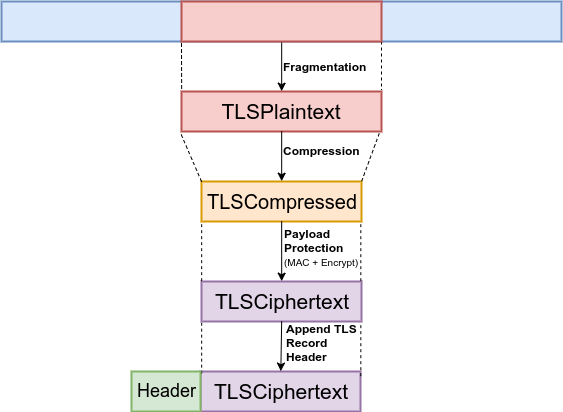
\includegraphics[width=1.0\textwidth]{img/tls-record-processing-3.png}
  \caption{\label{fig:tls-record-processing}TLS 1.2 Record Processing}
\end{figure}

The process described above, as well as the structure names are depicted in Figure \ref{fig:tls-record-processing}.
The compression step is not present in \gls{tls} 1.3. The structure names are exactly as the appear in the \gls{tls} specifications.

\subsection{\gls{tls} Keying Material} \label{keying}

In \gls{tls}, the confidentiality and integrity guarantees are achieved through the use
of \gls{sc}. Consequently, the communicating peers need to \textbf{share}
a \textbf{set of keys}. In \gls{tls} they are derived independently by the
client and the server, during the \gls{tls} Handshake Protocol.

The keys appear with different names in \gls{tls} $1.2$ and $1.3$ specs, but
they serve the same purpose. Additionally, more more keys can be found in
\gls{tls} $1.3$, for reasons that will be covered in Section \ref{tls-13}.
In \gls{tls} 1.2, the peers agree on the following set of keys:

\begin{itemize}
  \item \textit{client write key} - used by the client to encrypt the data to be sent
  \item \textit{client read key} - used by the client to decrypt the incoming data from the server
  \item \textit{server write key} - used by the server to encrypt the data to be sent
  \item \textit{server read key} - used by the server to decrypt the incoming data from the server
  \item \textit{client write IV} - used by the client for implicit nonce techniques with \gls{aead} ciphers
  \item \textit{server write IV} - used by the server for implicit nonce techniques with \gls{aead} ciphers
  \item \textit{client write MAC key} (\gls{tls} 1.2 only) - used by the client to authenticate the data to be sent
  \item \textit{client write MAC key} (\gls{tls} 1.2 only) - used by the client to authenticate the data to be sent
\end{itemize}

When communicating with one another, the client uses one key to
encrypt the data that it sends to the server and another key, different from the first one, to decrypt the data
that it receives from the server, and vice-versa. This implies that the  following relationships must hold:
\textit{client write key == server read key} and \textit{server write key == client read key}.

\subsection{TLS 1.2 Keying Material Generation} \label{keying-material}

The generation of secret keys, used for various cryptographic operations involves the
following steps, in order:

\begin{enumerate}
  \item Generate the \textbf{premaster secret}.
  \item From the \textbf{premaster secret} generate the \textbf{master secret}.
  \item From the \textbf{master secret} generate the various secret keys, which
  will be used in the cryptographic operations.
\end{enumerate}

The derivation of the keying material needed for a connection is done using
the \gls{tls} \gls{prf}. It is defined as \textit{PRF(secret, label, seed) = P\_hash(secret, label + seed)}.
The \textit{P\_hash(secret, seed)} function is an auxiliary data expansion function
which uses a single cryptographic hash function to expand a \textit{secret} and a \textit{seed}
into an arbitrary quantity of output. Therefore, it can be used to generate
anywhere from $1$ to an infinite number of bits of output. \textit{PRF(secret, label, seed)}
is used to generate as many bits of output as needed. When generating the
master secret, the \textit{secret} input is the \textit{premaster secret}.
When generating the key block, from which the final keys will be obtained,
the \textit{secret} input is the \textit{master secret}.

The cryptographic hash function used in \textit{P\_hash(secret, label, seed)} is
the hash function that is implicitly defined by the cipher suite in use. All of the cipher
suites defined in the \gls{tls} $1.2$ base spec use \textit{SHA-256} and any new
cipher suites must explicitly specify a the same hash function or a stronger one.

\subsection{TLS 1.2 Key Exchange Methods} \label{key-exchange}

The way the peremaster secret is generated depends on the key exchange
method used. This is the only phase of the keying material generation
phase that is variable for a fixed cipher suite, since a cipher suite defines
the \gls{prf} function that will be employed. Neither the derivation of the
shared keys are impacted by the key exchange method.

There are many key exchange methods to choose from. Some of them
are defined in the base spec (\textit{RFC5246}\cite{RFC5246}), while others
in separate \gls{rfc}s. For example, the \gls{ecc} based key exchange, specified
in \textit{RFC4492} \cite{RFC4492}).

The base spec specifies four key exchange methods, one using \gls{rsa} and
three using \gls{dh}:

\begin{itemize}
  \item static \gls{rsa} (\textit{RSA}; removed in \gls{tls} 1.3) - the client generates the premaster secret, encrypts it with the
  server's public key (which it obtained from the server's \textit{X.509} certificate) and
  sends it to the server. The server then decrypts it using the corresponding private key and uses it as its premaster secret. \gls{pfs} is
  a property that preserves the confidentiality of past interactions even if the
  long-term secret is compromised. This key exchange method offers authenticity, but does not offer \gls{pfs}.
  \item anonymous \gls{dh} (\textit{DH\_annon}; removed in \gls{tls} 1.3) -
  each run of the protocol, uses
  different pubic \gls{dh} parameters, which are generated dynamically. This results
  in a different, \textbf{ephemeral} key being generated every time. Since the exchanged \gls{dh}
  parameters are \textbf{not authenticated}, the resulting key exchange
  vulnerable to \gls{mitm} attacks. \gls{tls} $1.2$ spec states that cipher suites
  using \textit{DH\_annon} \textbf{must not} be used, unless the application
  layer explicitly requests so. This key exchange offers \gls{pfs}, but does not offer
  authenticity.
  \item fixed/static \gls{dh} (\textit{DH}; removed in \gls{tls} 1.3) - the server's/client's public \gls{dh} parameter
  is embedded in its certificate. This key exchange method offers authenticity,
  but does not offer \gls{pfs}.
  \item ephemeral \gls{dh} (\textit{DHE}) - the \gls{dh} protocol is used, identically to \textit{DH\_annon}, but the public parameters
  are digitally signed in some way, usually using the sender's private
  \gls{rsa} (\textit{DHE\_RSA}) or \gls{dsa} (\textit{DHE\_DSS}) key. This key
  exchange offers both, authenticity and \gls{pfs}.
\end{itemize}

When either of the \gls{dh} variants is used, the value obtained from the exchange is used
as the premaster secret. Usually, only the server's
authenticity is desired, but client's can also be achieved if it supplies the
server with its certificate. Whenever the server is authenticated, it is secure
against \gls{mitm} attacks. Table \ref{kemsp} summarizes the security properties
offered by each key exchange method.

\begin{table}[]
\centering
\caption{Key exchange methods and security properties}
\label{kemsp}
\begin{tabular}{|l|c|l|}
\hline
\textbf{Key Exchange Method} & \multicolumn{1}{l|}{Authentication} & PFS                    \\ \hline
RSA                          & X                                   &                        \\ \hline
DH\_anon                     & \multicolumn{1}{l|}{}               & \multicolumn{1}{c|}{X} \\ \hline
DH                           & X                                   &                        \\ \hline
DHE                          & X                                   & \multicolumn{1}{c|}{X} \\ \hline
\end{tabular}
\end{table}

In \gls{tls} $1.3$, static \gls{rsa} and \gls{dh} ciphersuites have been removed, meaning that all
public key exchange mechanisms now provide \gls{pfs}. Even though
anonymous \gls{dh} key exchange has been removed,
unauthenticated connections are still possible, by either using raw public keys\cite{RFC7250} or not verifying the certificate chain and any of its contents.

The use of \gls{ecc}-based key exchange (\gls{ecdh} and \gls{ecdhe}) and authentication (\gls{ecdsa})
algorithms with \gls{tls} is described in \textit{RFC4492}\cite{RFC4492}. The document introduces five new
\gls{ecc}-based key exchange algorithms, all of which use \gls{ecc} to compute
the premaster secret, differing only in whether the negotiated
keys are ephemeral (\gls{ecdh}) or long-term (\gls{ecdhe}), as well as the mechanism (if any) used to
authenticate them. Three new \gls{ecdsa} \textbf{client authentication} mechanisms are also defined,
differing in the algorithms that the certificate must be signed with, as well
as the key exchange algorithms that they can be used with.
Those features are negotiated through \gls{tls} extensions.

\subsection{TLS Extensions} \label{extensions}

\gls{tls} extensions were originally defined in \textit{RFC 4366}\cite{RFC4366}
and later merged into the \gls{tls} $1.2$ base spec. Each extension consists of an
extension type, which identifies the particular extension type, and extension data,
which contains information specific to a particular extension.

The extension mechanism can be used by \gls{tls} clients and servers; it is backwards
compatible, which means that the communication is possible between a \gls{tls} client that supports a particular extension and a server that does not support it,
and vice versa. A client may request the use of extensions by sending an extended \textit{ClientHello}
message, which is just a normal \textit{ClientHello} with an additional
block of data that contains a list of extensions. The backwards compatibility is achieved based on the \gls{tls}
requirement that the servers that are not extensions-aware must ignore the data
added to the \textit{ClientHello}s that they do not understand (section \textit{7.4.1.2} of \textit{RFC 2246}\cite{RFC2246}). Consequently,
even servers running older \gls{tls} versions that do not support extensions, will not break.

The presence of extensions can be determined by checking if there are bytes
following the \textit{compression\_methods} field in the \textit{ClientHello}.
If the server understands an extension, it sends back an extended \textit{ServerHello},
instead of a regular one. An extended \textit{ServerHello} is a regular
\textit{ServerHello} with an additional block of data following the
\textit{compression\_method}, containing a list of extensions.

An extended \textit{ServerHello} message can only be sent in a response to an
extended \textit{ClientHello} message. This prevents the possibility that an extended
\textit{ServerHello} message could cause a malfunction of older \gls{tls} clients that do not
support extensions. An extension type must not appear in the
extended \textit{ServerHello}, unless the same extension type appeared in the
corresponding extended \textit{CleintHello}, and if this happens, the client must abort the handshake.

\subsection{TLS 1.3} \label{tls-13}

Due to limited space, \gls{tls} $1.3$\cite{I-D.ietf-tls-tls13} will not be described in detail. 
The focus was on \gls{tls} $1.2$ instead, because at the time the work on the thesis started, 
\gls{tls} $1.3$ is still in draft mode and $1.2$ was the latest and the recommended to use version.

Numerous differences from \gls{tls} $1.3$ to $1.2$ have been mentioned throughout the document.
Various characteristics found in \gls{tls} $1.3$ make it more suitable for the context
of \gls{iot} than \gls{tls} $1.2$. Some of them were already mentioned previously, and in this section a additional ones will be outlined.

The first important difference is that the use of extensions is required in \gls{tls} $1.3$.
This can be explained by the fact that some of the functionality has been moved into extensions, in order to preserve
backwards-compatibility with the \textit{ClientHello}s of the previous versions.
The way a server distinguishes if a client is requesting \gls{tls} $1.3$
is by checking the presence of the \textit{supported\_versions} extension in the
extended \textit{ClientHello}.

In \gls{tls} $1.3$ more data is encrypted and the encryption begins earlier. For example,
at the server-side there is a notion of "encrypted extensions". The \textit{EncryptedExtensions}
message, as the name suggests, contains a list of extensions that are encrypted
under a symmetric key. It contains any extensions that are not needed
for the establishment of the cryptographic context.

One of the main problems with using \gls{tls} in \gls{iot} is that while \gls{iot}
traffic needs to be quick and lightweight, \gls{tls} $1.2$ adds two additional
round trips (\textit{2 RTT}) to the start of every session. \gls{tls} $1.3$ handshake has a lower latency,
and this is extremely important in the context of \gls{iot}.
The full \gls{tls} $1.3$ handshake is only \textit{1 RTT}. \gls{tls} $1.3$ even allows
clients to send data on the first flight (known as \textbf{early client data}), when the clients
and servers share a \gls{psk} (either obtained externally or via a previous handshake).
This means that in \gls{tls} $1.3$ \textit{0-RTT} data is possible, by
encrypting it with a key derived from a \gls{psk}. Session resumption
via identifiers and tickets has been obsoleted in \gls{tls} $1.3$, and both methods
have been replaced by a \gls{psk} mode. This \gls{psk} is established in a previous
connection after the handshake is completed and can be presented by the client
on the next visit.

Keying material generation is more complex in \gls{tls} $1.3$ than in
\gls{tls} $1.2$, since different
keys are used to encrypt data throughout the Handshake protocol. This can be
explained by the fact that in \gls{tls} $1.3$ the encryption begins earlier.
Other Handshake messages besides \textit{Finished} are encrypted. As a result,
multiple encryption keys are generated and used to encrypt different data
throughout the handshake.

The way the keying material is derived is also different. The
\gls{prf} construction described above has been replaced.
In \gls{tls} 1.3, key derivation uses the
\gls{hkdf} function \cite{RFC5869} and its two components: \textit{HKDF-Extract} and \textit{HKDF-Expand}.
This new design allows easier analysis by cryptographers due to improved
key separation properties.

%
\subsection{\gls{dtls}} \label{dtls}

As already mentioned, \gls{dtls} is an adaption of \gls{tls} that runs on
top of an unreliable transport protocol, such as UDP. The design of \gls{dtls} is deliberately very similar to \gls{tls}, in fact, its specification is written
in terms of differences from \gls{tls}. This similarity allows to
both, minimize new security invention, and maximize the amount of code and infrastructure reuse. The changes are mostly done at the lower level and
don not affect the core of the protocol.
Even extensions defined before \gls{dtls} existed can be
used with it. The latest version of \gls{dtls} is $1.2$ and it is defined
in \textit{RFC 6347}\cite{RFC6347}. There is a draft of \gls{dtls} $1.3$
\cite{I-D.ietf-tls-dtls13} that is currently under active development.

Since \gls{dtls} operates on top of an unreliable transport protocol, such as
UDP, it must explicitly deal with the absence of reliable and ordered assumptions
that are made by \gls{tls}. The main differences from \gls{dtls} $1.2$ to \gls{tls} $1.2$ are:

\begin{itemize}
  \item two new fields are added to the record layer: an explicit \textit{2 byte} sequence
  number and a \textit{6 byte} epoch. The \gls{dtls} \gls{mac} is the same as in \gls{tls},
  however, rather than using the implicit sequence number, the \textit{8 byte} value
  formed by concatenation of the epoch number and the sequence number is used.

  \item stream ciphers must not be used with \gls{dtls}.

  \item a stateless cookie exchange mechanism has been added to the handshake protocol
  in order to prevent \gls{dos} attacks. To accomplish this, a new handshake
  message, the \textit{HelloVerifyRequest} has been added. After
  the \textit{ClientHello}, the server responds with a \textit{HelloVerifyRequest}
  containing a cookie, which is returned back to the server in another
  \textit{ClientHello} that follows it. After this, the handshake proceeds as in \gls{tls}. This is depicted in Figure \ref{fig:dtls-cookie}.   Although optional for the server, this mechanism highly recommended, and the
  client must be prepared to respond to it. \gls{dtls} $1.3$ follows the same idea, but does it differently, namely,
  the \textit{HelloVerifyRequest} message has been removed, and the cookie is conveyed to the client via an extension in a \textit{HelloRetryRequest} message.

  \item the handshake message format has been extended to deal with message reordering,
  fragmentation and loss by addition of three new fields: a message sequence field,
  a fragment offset field and a fragment length field.
\end{itemize}

\section{Related Work} \label{related-work}

Lightweight cryptography is an important topic in the context of \gls{iot} security, due to the resource-limited nature of the devices. This section will begin with the description of the work done in this area.

Biryukov \textit{et al}\cite{Stateoft96:online} explore the topic of lightweight symmetric cryptography,
providing a summary of the lightweight symmetric
primitives from the academic community, the government agencies and even proprietary
algorithms which have been either reverse-engineered or leaked. All of those algorithms
are listed in the paper, alongside relevant metrics. The list will not be
included herein due to the lack of space. The authors also proposed
to split the field into two areas: ultra-lightweight and \gls{iot} cryptography.

The paper systematizes the knowledge in the area oe lightweight cryptography
in order to define "lightweightness" more precisely. The authors observed that the design
of lightweight cryptography algorithms varies greatly, the only unifying thread
between them being the low computing power of the devices that they are designed for.

The most frequently optimized metrics are the memory consumption, the implementation size
and the speed or the throughput of the primitive. The specifics depend on whether
the hardware or the software implementations of the primitives are considered.

If the primitive is implemented in hardware, the memory consumption and the implementation
size are lumped together into its gate area, which is measured in Gate Equivalents (GE),
a metric quantifying how physically large a circuit implementing the primitive is.
The throughout is measured in \textit{bytes/sec} and it corresponds to the amount of plaintext
processed per time unit. If a primitive is implemented in software (typically for
use in micro-controllers), the relevant metrics are the RAM consumption, the code
size and the throughput of the primitive, measured in \textit{bytes/CPU cycle}.

To accommodate the limitations of the constrained devices, most lightweight algorithms
are designed to use smaller internal states with smaller key sizes. After analysis,
the authors concluded that even though at least \textit{128 bit} block and
key sizes were required from the AES candidates, most of the lightweight
block ciphers used only \textit{64-bit} blocks, which leads to a smaller memory
footprint in both, software and hardware, while also making the algorithm better suited
for processing of smaller messages.

Even though algorithms can be optimized in implementation: whether it is
a software or a hardware, dedicated lightweight algorithms are still needed.
This comes down mainly to two factors: there are limitations to the the extent of
the optimizations that can be done and the hardware-accelerated encryption is
frequently vulnerable to various \gls{sca}s. An example of such an attack is the one done on the
Phillips light bulbs \cite{cryptoeprint:2016:1047}, where the authors were able to
recover a secret key used to authenticate updates.

It is more difficult to implement a lightweight hash function than a lightweight
block cipher, since standard hash functions need large amounts
of memory to store both: their internal states, for example, \textit{1600 bits} in case of SHA-3,
and the block they are operating on, for example, \textit{512 bits} in the case of SHA-2.
The required internal state is acceptable for a desktop computer, but not for a
constrained device. Taking this into consideration, the most common approach
taken by the designers is to use a sponge construction with a very small bitrate.
A sponge function is an algorithm with an internal state that takes as an input
a bit stream of any length and outputs a bit stream of any desired length. Sponge
functions are used to implement many cryptographic primitives, such as cryptographic
hashes. The bitrate decides how fast the plain text is processed and how fast the
final digest is produced. A smaller bitrate means that the output will take longer
to be produced, which means that a smaller capacity (the security level)
can be used, which minimizes the memory footprint at the cost of slower data
processing. A capacity of \textit{128 bits} and a bitrate of \textit{8 bits}
are common values for lightweight hash functions.

Another trend in the lightweight algorithms noticed by the authors is the
preference for \textit{ARX}-based and \textit{bitsliced-S-Box} based designs, as well as simple key schedules.

Finally, a separation of the "lightweight algorithm" definition into two distinct fields has been proposed:

\begin{itemize}
  \item \textbf{Ultra-Lightweight Crypto} - algorithms running on very cheap
  devices \textbf{not connected to the internet}, which are easily replaceable
  and have a limited life-time. Examples: \textit{RFID} tags, smart cards and remote car keys.
  \item \textbf{IoT Crypto} - algorithms running on a low-power device,
  \textbf{connected to a global network}, such as the internet. Examples: security cameras, smart light bulbs and smart watches.
\end{itemize}

Considering the two definitions above, this the work of this dissertation focuses on \textbf{IoT Crypto}
devices. A summary of differences between the both categories is summarized in
table \ref{ul-iot}.

\begin{table}[]
\centering
\caption{A summary of the differences between ultra-lightweight and IoT crypto}
\label{ul-iot}
\begin{tabular}{@{}lll@{}}
\toprule
                           & \textbf{Ultra-Lightweight}          & \textbf{IoT}                           \\ \midrule
\textbf{Block Size}        & 64 bits                             & ≥ 128 bits                             \\
\textbf{Security Level}    & ≥ 80 bits                           & ≥ 128 bits                             \\
\textbf{Relevant Attacks}  & low data/time complexity            & same as "regular" crypto               \\
\textbf{Intended Platform} & dedicated circuit (ASIC, RFID...)   & micro-controllers, low-end CPUs        \\
\textbf{SCA Resilience}    & important                           & important                              \\
\textbf{Functionality}     & one per device, e.g. authentication & encryption, authentication, hashing... \\
\textbf{Connection}        & temporary, only to a given hub      & permanent, to a global network         \\ \bottomrule
\end{tabular}
\end{table}

While there is a high demand for lightweight public key primitives, the required
resources for them are much higher than for symmetric ones. As a
paper by Katagi \textit{et al}\cite{b5b8db9716:online}
concluded, there are no promising primitives
that have enough lightweight and security properties, compared to the
conventional ones, such as RSA and \gls{ecc}. Further research on this topic, as part of the work on this dissertation, lead to the same conclusion.

Lightweight cryptography is an important topic this work and there are papers detailing
various algorithms. In order to provide a good overview of it while staying succinct, recent papers that provide a summary of the
area, rather than focusing on specific implementations, were chosen.
The remainder of this section will focus on the work done on the (D)\gls{tls} protocol in the context of \gls{iot}.

The "Scalable Security With Symmetric Keys"\cite{S3KScala62:online} paper proposes a key management architecture for resource-constrained devices,
which allows devices that have no previous, direct security relation to use
(D)\gls{tls} using one of two approaches: shared symmetric keys or raw public keys.
The resource-constrained device is a server that offers one or more resources,
such as temperature readings. The idea in both approaches is to introduce a third-party
\textit{trust anchor (TA)} that both, the client and the server use to establish
trust relationships between them.

The first approach is similar to Kerberos\cite{RFC4120}, and it does not require any
changes to the original protocol. A client can request a \gls{psk} \textit{Kc} from the \textit{TA},
which will generate it and send it back to the client via a secure channel, alongside
a \textit{psk\_identity} which has the same meaning and use as in \textit{RFC 4279}\cite{RFC4279}. When connecting to the server,
the client will send to the server the \textit{psk\_identity} that it received in a previous
handshake. Upon its receipt, the server will derive the \textit{Kc}, using the
\textit{P\_hash()} function defined in \textit{RFC 5246}\cite{RFC5246}.

The second approach consists in requesting an \gls{apk}
from the \textit{TA}. The client includes his \gls{rpk} in its request, which is used for authorization. The TA
creates an authorization certificate, protects it with a \gls{mac} and sends it
to the client alongside the server's public key.
The client then sends this \gls{apk} (instead of the \gls{rpk})
when connecting to the server, which verifies it (to authorize the client)
and proceeds with the handshake in the \gls{rpk} mode, as defined in \textit{RFC 4279} \cite{RFC4279}.
To achieve this, a new certificate structure is defined, alongside a new \textit{certificate\_type}.
The new certificate structure is just the \textit{RFC7250} \cite{RFC7250} structure, with an
additional \gls{mac}.

The hash function used for key derivation is SHA256. The authors evaluated the
performance of their solution with and without SHA2 hardware acceleration and
concluded that while it had significant impact on key derivation, it had little
impact on the total handshake time (\textit{711.11 ms} instead of \textit{775.05 ms}), since most of the time was spent in sending
data over the network and other parts of the handshake, the longest one being
the \textit{ChangeCipherSpec} message which required a processing time
of \textit{17.79ms}.

6LoWPAN\cite{RFC4944} is a protocol that allows devices with limited processing
ability and power to transmit information wirelessly using the \textit{IPv6}
protocol. The protocol defines IP Header Compression (IPHC) for the IP header, as well as,
Next Header Compression (NHC) for the IP extension headers and the UDP header in \textit{RFC 6282}\cite{RFC6282}.
The compression relies on the shared context between the communicating peers.

The work proposed in \cite{6LoWPANC53:online} uses this same idea, but with the goal of compressing \gls{dtls} headers.
6LoWPAN does not provide ways to compress the UDP payload and layers above.
A proposed standard\cite{RFC7400} for generic header compression
for 6LoWPANs that can be used to compress the UDP payload, does exit, however. The authors propose
a way to compress \gls{dtls} headers and messages using this mechanism.

Their work defines how the \gls{dtls} Record header, the \gls{dtls} Handshake header,
the \textit{ClientHello} and the \textit{ServerHello} messages can be compressed, but notes that
the same compression techniques can be used to compress the remaining handshake
messages. They explore two cases for the header compression: compressing both,
the Record header and the Handshake header and compressing the Record header only,
which is useful after the handshake has completed and the fragment field of the
Record layer contains application data, instead of a handshake message.

\begin{figure}
  \centering
  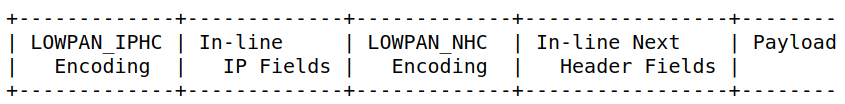
\includegraphics[width=0.9\textwidth]{img/6lowpan-header.png} % first figure
  itself
\caption{\label{fig:6lowpan-header} IPv6 Next Header Compression}
\end{figure}

\begin{figure}
  \centering
  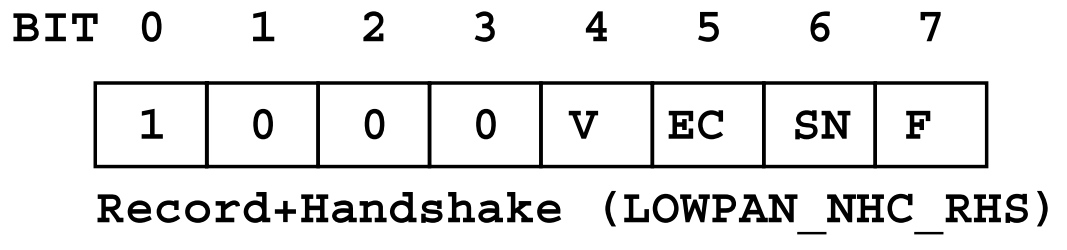
\includegraphics[width=0.6\textwidth]{img/6lowpan-ghc-rhs.png} % second figur
  e itself
  \caption{\label{fig:6lowpan-ghc-rhs} LOWPAN\_NHC\_RHS structure}
\end{figure}


Each \gls{dtls} fragment is carried over as a UDP payload. In this case,
the UDP payload carries a header-like payload (the \gls{dtls} record header).
Figure \ref{fig:6lowpan-header} shows the way IPv6 next header compression is done.
The authors use the same value for the \textit{LOWPAN\_NHC Encoding} field (defined in \textit{RFC 6282}\cite{RFC6282})
as in \textit{RFC7400} and define the format of the \textit{In-line Next Header Fields}
(also defined in \cite{RFC6282}), which is the compressed \gls{dtls} content. The \textit{LOWPAN\_IPHC Encoding}
and \textit{In-Line IP Fields} fields are used in the IPv6 header compression
and are not in the scope of the paper.

All of the cases follow the same basic idea, for this reason only one of them will be exemplified:
the case where both, the Record and the Handshake headers are compressed.
In this case \textit{LOWPAN\_NHC Encoding} will contain the \textit{LOWPAN\_NHC\_RHS}
structure (depicted in figure \ref{fig:6lowpan-ghc-rhs}), which is the compressed form of the Record and Handshake headers. The
parts that are not compressed will be contained in the \textit{Payload} part.
The first four bits represent the ID field and in this case they are fixed to \textit{1000},
that way, the decompressor knows what is being compressed (\textit{i.e} how to interpret
the structure that follows the ID bits). If the \textit{F} field of the \textit{LOWPAN\_NHC\_RHS} structure contains the
bit \textit{0}, it means that the handshake message is not fragmented, so
the \textit{fragment\_offset} and \textit{fragment\_length} fields are
elided from the Handshake header (common case when a handshake message is not bigger than
the maximum header size), meaning that they are not going to be sent at
all (\textit{i.e.} they are not going to be present in the \textit{Payload} part).
If the \textit{F} bit has the value \textit{1}, the \textit{fragment\_offset}
and \textit{fragment\_length} fields are carried inline (\textit{i.e.} they are
present in the \textit{Payload} part). The remaining two fields define similar
behavior for other header fields (some of them assume that some default value is present, when a field is elided).
The \textit{length} field in the Record and Handshake headers are always elided,
since they can be inferred from the lower layers.

The evaluation showed that the compression can save a significant number of bits:
the Record header, that is included in all messages can be compressed by \textit{64 bits}
(\textit{i.e.} by $62\%$).

There is also a proposal for TCP header compression for 6LoWPAN\cite{I-D.aayadi-6lowpan-tcphc},
which if adopted, in many cases can compress the mandatory \textit{20 bytes} TCP header
into \textit{6 bytes}. This means that the same ideas can be applied to TCP and
\gls{tls} as well.

Later, in 2013, Raza \textit{et al.} proposed a security scheme called Lithe\cite{LitheLig40:online},
which is a lightweight security solution for \gls{coap} that uses the same \gls{dtls} header
compression technique as in \cite{6LoWPANC53:online} with the goal of implementing
it as a security support for \gls{coap}. \gls{coap}\cite{RFC7959} is a specialized
\textit{REST}ful Internet Application Protocol for constrained devices. it is designed to easily
translate to HTTP, in order to simplify its integration with the web,
while also meeting requirements such as multicast support and low overhead.
\gls{coap} is like "HTTP for constrained devices".
It can run on most devices that support UDP or a UDP-like protocol.
\gls{coap} mandates the use of \gls{dtls} as the underlying security protocol for
authenticated and confidential communication. There is also a \gls{coap} specification
running on top of TCP, which uses \gls{tls} as its underlying security protocol
currently being developed\cite{I-D.ietf-core-coap-tcp-tls}.

The authors evaluated their system in a simulated environment in \textit{Contiki OS}\cite{ContikiT75:online}, which is an open-source operating system for the \gls{iot}.
They obtained significant gains in terms of packet size (similar numbers to the
ones observed in \cite{6LoWPANC53:online}), energy consumption (on average $15\%$ less
energy is used to transmit and receive compressed packets), processing time
(the compression and decompression time of \gls{dtls} headers is almost negligible)
and network-wide response times (up to $50\%$ smaller RTT). The
gains in the mentioned measures are the largest when the compression avoids
fragmentation (in the paper, for payload size of \textit{48 bytes}).

Angelo \textit{et al.} \cite{Security5:online} proposed to integrate the \gls{dtls} protocol
inside \gls{coap}, while also exploiting \gls{ecc} optimizations and minimizing
ROM occupancy. They implemented their solution in an off-the-shelf mote platform
and evaluated its performance. \gls{dtls} was designed to protect web application communication, as a result,
it has a big overhead in \gls{iot} scenarios. Besides that, it runs over UDP,
so additional mechanisms are needed to provide the reliability and ordering
guarantee. With this in mind, the authors wanted to design a version of \gls{dtls}
that both: minimizes the code size and the number of exchanged messages, resulting
in an optimized Handshake protocol.

In order to minimize the code size occupied by the \gls{dtls} implementation, they
decided to delegate the tasks of \textbf{reliability} and \textbf{fragmentation} to
\gls{coap}. This means that the code responsible for those functionalities,
can be removed altogether from the \gls{dtls} implementation, thus reducing ROM
occupancy. This part of their work was based on an informational RFC draft\cite{I-D.keoh-dtls-profile-iot}, in which the
authors profiled \gls{dtls} for \gls{coap}-based \gls{iot} applications and proposed
the use of a \textit{RESTful} \gls{dtls} handshake which relies on \gls{coap} block-wise
transfer to address the fragmentation issue.

To achieve this they  proposed the use of a \textit{RESTful} \gls{dtls} connection as a \gls{coap} resource,
which is created when a new secure session is requested.
The authors exploit the the \gls{coap}s capability to provide connection-oriented
communication offered by its message layer. In particular, each \textit{Confirmable}
\gls{coap} message requires an \textit{Acknowledgement} message (page 8 of \textit{RFC 7252} \cite{RFC7252}),
which acknowledges that a specific \textit{Confirmable} message has arrived, thus
providing reliable retransmission.

Instead of leaving the fragmentation function to \gls{dtls}, it was
delegated to the block-wise transfer feature of \gls{coap}\cite{RFC7959}, which was developed
to support transmission of large payloads. This approach has two advantages: first, the code in the \gls{dtls}
layer responsible for this function can be removed, thus reducing ROM occupancy,
and second, the fragmentation/reassembly process burdens the lower layers
with state that is better managed in the application layer.

The authors also optimized the implementation of basic operations on which
many security protocols, such as \gls{ecdh} and \gls{ecdsa} rely upon. The first
optimization had to do with modular arithmetic on large integers. A set of optimized
assembly routines based on \cite{Comparin25:Online} allow the improved use of
registers, reducing the number of memory operations needed to perform
tasks such as multiplications and square roots on devices with \textit{8-bit} registers.

Scalar multiplication is often the most expensive operation in \gls{ec}-based
cryptography, therefore optimizing it is of high interest. The authors used a
technique called \textit{IBPV} described in \cite{LowcostS87:online}, which is based on pre-computation.
of a set of discrete log pairs. The mathematical details have been purposefully omitted,
since they are not relevant for this description. The \textit{IBPV} technique was used
to improve the performance of the \gls{ecdsa} signature and extended to the
\gls{ecdh} protocol. In order to reduce the time taken to perform an \gls{ecdsa}
signature verification, the \textit{Shamir Trick} was used, which allows
to perform the sum of two scalar multiplications (frequent operation in \gls{ec} cryptography)
faster than performing two independent scalar multiplications.

The results showed that the \gls{ecc} optimizations
outperform the scalar multiplication in the state of the art class 1 device platforms,
while also improving the the network lifetime by a factor of up to $6.5$ with
respect to a standard, non-optimized implementation. Leaving reliability and
fragmentation tasks to \gls{coap}, reduces the \gls{dtls} implementation code size
by approximately $23\%$.

\textit{RFC 7925}\cite{RFC7925} describes a \gls{tls} and \gls{dtls} $1.2$
profile for \gls{iot} devices that offer communication security services
for \gls{iot} applications.
In this context, "profile" means available configuration options (ex: which
cipher suites to use) and protocol extensions that are best suited for \gls{iot} devices.
The document is rather lengthy, only its fundamental parts will be summarized. A number of relevant \gls{rfc}s will also be described.

\textit{RFC 7925} explores both cases: constrained clients and constrained servers, specifying
a profile for each one and describing the main challenges faced in each scenario.
The profile specifications for constrained clients and servers are very similar.
Code reuse in order to minimize the implementation size is recommended. For example, an \gls{iot} device
using a network access solution based on \gls{tls}, such as EAP-TLS\cite{rfc5216}
can reuse most parts of the code for (D)\gls{dtls} at the application layer.

For the credential types the profile considers 3 cases:

\begin{itemize}
  \item \gls{psk} - authentication based on \gls{psk}s is described in
  \textit{RFC 4249}\cite{RFC4279}. When using \gls{psk}s, the client indicates which
  key it wants to use by including a \gls{psk} identity in its \textit{ClientKeyExchange} message.
  A server can have different \gls{psk} identities shared with different clients.
  An identity can have any size, up to a maximum of \textit{128 bytes}.
  The profile recommends the use of shorter \gls{psk} identities and specifies
  \textit{TLS\_PSK\_WITH\_AES\_128\_CCM\_8} as the only mandatory-to-implement
  cipher suite to be used with \gls{psk}s, just like \gls{coap} does. If a \gls{pfs} cipher suite is used, ephemeral
  \gls{dh} keys should not be reused over multiple protocol exchanges.

  \item \gls{rpk} - the use of \gls{rpk}s in (D)\gls{tls} is described in \textit{RFC 7250}\cite{RFC7250}.
  With \gls{rpk}s, only a subset of the information that is found in typical certificates
  is used: namely the \textit{SubjectPublicKeyInfo} structure, which contains
  the necessary parameters to describe the public key (the algorithm identifier
  and the public key itself). Other PKIX certificate\cite{RFCabc} parameters are
  omitted, making the resulted \gls{rpk} smaller in size, when compared to the
  original certificate and the code to process the keys simpler. In order for the
  peers to negotiate a \gls{rpk}, two new extensions have been defined:
  one for the client indicate which certificate types it can provide to the server, and one to indicate which certificate types it can process from the server. To further reduce the size of the implementation, the profile
  recommends the use of the \gls{tls} Cached Information extension\cite{RFC7924}, which
  enables \gls{tls} peers to exchange just the fingerprint (a shorter sequence of bytes
  used to identify a public key) of the public key. Identical to \gls{coap}, the only mandatory-to-implement
  cipher suite to be used with \gls{rpk}s is \textit{TLS\_ECDHE\_ECDSA\_WITH\_AES\_128\_CCM\_8}.

  \item certificate - conventional certificates can also be used. The support
  for the Cached Information extension\cite{RFC7924} and the\\ \textit{TLS\_ECDHE\_ECDSA\_WITH\_AES\_128\_CCM\_8}
  cipher suite is required. The profile restricts the use of named curves to
  the ones defined in \textit{RFC 4492}\cite{RFC4492}. For certificate revocation, neither the
  \gls{ocsp}\cite{RFC6960}, nor the \gls{crl}\cite{RFCabc} mechanisms are used, instead this task is delegated to
  the software update functionality. The Cached Information extension does not
  provide any help with caching client certificates. For this reason, in cases
  where client-side certificates are used and the server is not constrained,
  the support for client certificate URLs is required. The client certificates URL
  extension\cite{RFC4366} allows the clients to point the server to a URL from
  which it can obtain its certificate, which allows constrained clients to
  save memory and amount of transmitted data. The Trusted CA Indication\cite{RFC6066}
  extension allows the clients to indicate which trust anchors they support, which is useful
  for constrained clients that due to memory limitation posses only a small number
  of \gls{ca} root keys, since it can avoid repeated handshake failures. If the clients interacts with
  dynamically discovered set of (D)\gls{tls} servers, the use of this extension is recommended,
  if that set is fixed, it is not.

\end{itemize}

The signature algorithms extension\cite{RFC5246} allows the client to indicate
to the server which signature/hash pairs it supports to be used with digital signatures.
The client must send this extension to indicate the use of \textit{SHA-256},
otherwise the defaults defined in \cite{RFC5246} are used. This extension is not
applicable when \gls{psk}-based cipher suites are used.

The profile mandates that constrained clients must implement session
resumption to improve the performance of the handshake since this will lead to
less exchanged messages, lower computational overhead (since only symmetric cryptography
is used) and it requires less bandwidth. If server is constrained, but
the client is not, the client must implement the Session Resumption Without
Server-Side State mechanism\cite{RFC5077}, which is achieved through the
use of tickets. The server encapsulates the state into a ticket and forwards it to
the client, which can subsequently resume the session by sending back that ticket.
If both, the client and the server are constrained, both of them should implement
\textit{RFC 5077}\cite{RFC5077}.

The use of compression is not recommended for two reasons. First, \textit{RFC7525}\cite{RFC7525}
recommends disabling (D)\gls{tls} level compression, due to attacks such as \textit{CRIME}\cite{Microsof72:online}.
\textit{RFC7525} provides recommendations for improving the security of deployed services
that use \gls{tls} and \gls{dtls} and was published as a response to the various
attacks on (D)\gls{tls} that have emerged over the years. Second, for \gls{iot} applications,
the (D)\gls{tls} compression is not needed, since application-layer protocols are highly
optimized and compression at the (D)\gls{tls} layer increases the implementation's size and complexity.

\textit{RFC6520}\cite{RFC6520} defines a heartbeat mechanism to test whether the peer
is still alive. The implementation of this extension is recommended for server
initiated messages. Note that since the messages sent to the client will most likely
get blocked by middleboxes, the initial connection setup is initiated by the
client and then kept alive by the server.

Random numbers play an essential role in the overall security of the protocol.
Many of the usual sources of entropy, such as the timing of keystrokes and the
mouse movements, will not be available on many \gls{iot} devices, which means that
either alternative ones need to be found or dedicated hardware must be added.
\gls{iot} devices using (D)\gls{tls} must be able to find entropy sources adequate for the generation of quality
random numbers, the guidelines and requirements for which can be found in \textit{RFC4086}\cite{rfc4086}.

Implementations compliant with the profile must use \gls{aead} ciphers, therefore
encryption and \gls{mac} computation are no longer independent steps, which means
that neither encrypt-then-MAC\cite{RFC7366}, nor the truncated MAC\cite{RFC6066} extensions are applicable
to this specification and must not be used.

The \gls{sni} extension\cite{RFC6066} defines a mechanism for a client to
tell a (D)\gls{tls} server the name of the server that it is contacting. This is
crucial in case when multiple websites are hosted under the same IP address.
The implementation of this extension is required, unless the (D)\gls{tls}
client does not interact with a server in a hosting environment.

The maximum fragment length extension\cite{RFC6066} lowers the maximum fragment
length support of the record layer from $2^14$ to $2^9$. This extension allows
the client to indicate the server how much of the incoming data it is able to buffer,
allowing the client implementations to lower their RAM requirements, since it does not
not need to accept packets of large size, such as the \textit{16K} packets required by
plain (D)\gls{tls}. For that reason, client implementations must support this
extension.

The Session Hash Extended Master Secret Extension\cite{RFC7627} defines an extension
that binds the master secret to the log of the full handshake, thus preventing
\gls{mitm} attacks, such as the triple handshake\cite{TripleHa89:online}. Even though the
cipher suites recommended by the profile are not vulnerable to this attack, the
implementation of this extension is advised. In order to prevent the renegotiation
attack\cite{RFC5746}, the profile requires the \gls{tls} renegotiation feature
to be disabled.

With regards to the key size recommendations, the authors recommend symmetric keys
of at least \textit{112 bit}, which corresponds to a \textit{233-bit} \gls{ecc}
key and to a \textit{2048} \gls{dh} key. Those recommendations are made
conservatively under the assumption that \gls{iot} devices have a long expected
lifetime ($10+$ years) and that those key recommendations refer to the long-term
keys used for device authentication. Keys that are provisioned dynamically
and used for protection of transactional data, such as the ones used in
(D)\gls{tls} cipher suites, may be shorter, depending on the sensitivity of
transmitted data.

Even though \gls{tls} defines a single stream cipher: \textit{RC4}, its use is no longer
recommended due to its cryptographic weaknesses described in \textit{RFC 7465}\cite{RFC7465}.

\textit{RFC 7925}\cite{RFC7925} points out that designing a software
update mechanism into an \gls{iot} system is crucial to ensure that potential vulnerabilities
can be fixed and that the functionality can be enhanced. The software update mechanism
is important to change configuration information, such as trust anchors and
other secret-key related information. Although the profile refers to \textit{LM2M}\cite{OpenMobi29:online}
as an example of protocol that comes with a suitable software update mechanism,
there has been new work done in this area since the release of this profile.
There is a document specifying an architecture for a firmware update
mechanism for \gls{iot} devices\cite{I-D.moran-suit-architecture} currently in Internet-Draft state. % file "Thesis_Background.tex"
\cleardoublepage

%%%%%%%%%%%%%%%%%%%%%%%%%%%%%%%%%%%%%%%%%%%%%%%%%%%%%%%%%%%%%%%%%%%%%%%%%
%                                                                      %
%     File: Thesis_Implementation.tex                                  %
%     Tex Master: Thesis.tex                                           %
%                                                                      %
%     Author: Andre C. Marta                                           %
%     Last modified :  2 Jul 2015                                      %
%                                                                      %
%%%%%%%%%%%%%%%%%%%%%%%%%%%%%%%%%%%%%%%%%%%%%%%%%%%%%%%%%%%%%%%%%%%%%%%%

\chapter{Implementation}
\label{chapter:implementation}

Insert your chapter material here...

%%%%%%%%%%%%%%%%%%%%%%%%%%%%%%%%%%%%%%%%%%%%%%%%%%%%%%%%%%%%%%%%%%%%%%%%
\section{Numerical Model}
\label{section:model}

Description of the numerical implementation of the models explained in Chapter~\ref{chapter:background}...


%%%%%%%%%%%%%%%%%%%%%%%%%%%%%%%%%%%%%%%%%%%%%%%%%%%%%%%%%%%%%%%%%%%%%%%%
\section{Verification and Validation}
\label{section:verification}

Basic test cases to compare the implemented model against other numerical tools (verification) and experimental data (validation)...

 % file "Thesis_Implementation.tex"
%\cleardoublepage

%\input{Thesis_new_file} % add new .tex files for new chapters
% \cleardoublepage

%\input{Thesis_new_file} % add new .tex files for new chapters
% \cleardoublepage

%\input{Thesis_new_file} % add new .tex files for new chapters
% \cleardoublepage

%%%%%%%%%%%%%%%%%%%%%%%%%%%%%%%%%%%%%%%%%%%%%%%%%%%%%%%%%%%%%%%%%%%%%%%%
%                                                                      %
%     File: Thesis_Results.tex                                         %
%     Tex Master: Thesis.tex                                           %
%                                                                      %
%     Author: Andre C. Marta                                           %
%     Last modified :  2 Jul 2015                                      %
%                                                                      %
%%%%%%%%%%%%%%%%%%%%%%%%%%%%%%%%%%%%%%%%%%%%%%%%%%%%%%%%%%%%%%%%%%%%%%%%

\chapter{Results}
\label{chapter:results}

Insert your chapter material here...


%%%%%%%%%%%%%%%%%%%%%%%%%%%%%%%%%%%%%%%%%%%%%%%%%%%%%%%%%%%%%%%%%%%%%%%%
\section{Problem Description}
\label{section:problem}

Description of the baseline problem...


%%%%%%%%%%%%%%%%%%%%%%%%%%%%%%%%%%%%%%%%%%%%%%%%%%%%%%%%%%%%%%%%%%%%%%%%
\section{Baseline Solution}
\label{section:baseline}

Analysis of the baseline solution...


%%%%%%%%%%%%%%%%%%%%%%%%%%%%%%%%%%%%%%%%%%%%%%%%%%%%%%%%%%%%%%%%%%%%%%%%
\section{Enhanced Solution}
\label{section:enhanced}

Quest for the optimal solution...


% ----------------------------------------------------------------------
\subsection{Figures}
\label{subsection:figures}

Insert your section material and possibly a few figures...

Make sure all figures presented are referenced in the text!


% ----------------------------------------------------------------------
\subsubsection{Images}
\label{subsection:images}

\begin{figure}[!htb]
  \centering
  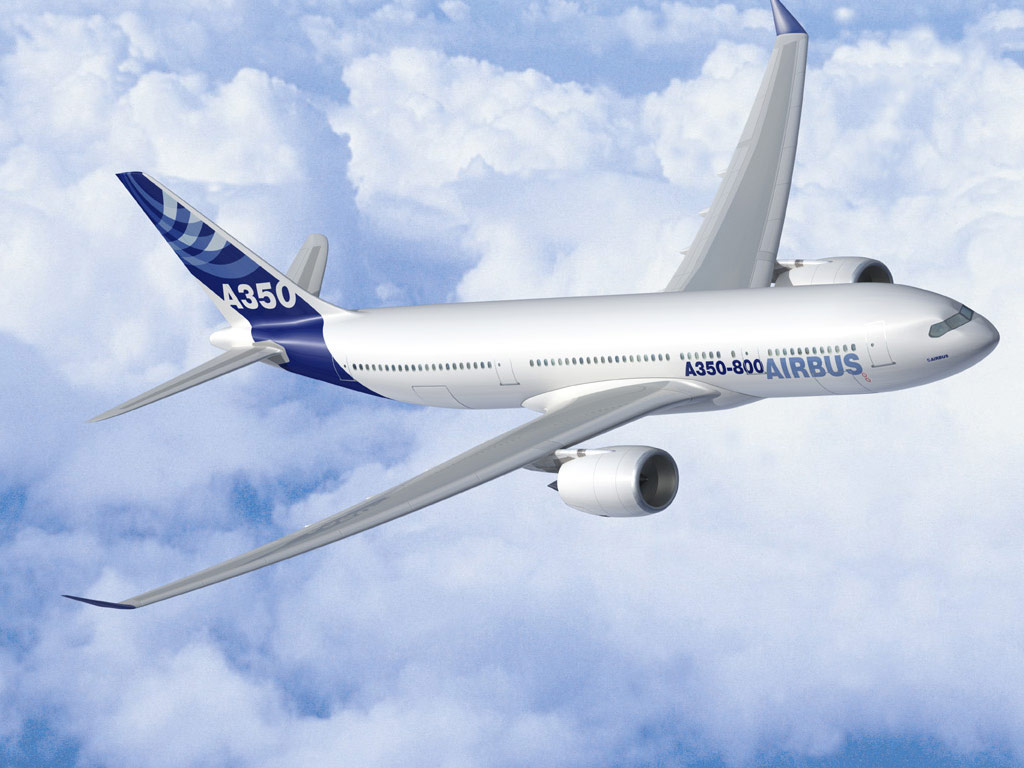
\includegraphics[width=0.25\textwidth]{Figures/Airbus_A350.jpg}
  \caption[Caption for figure in TOC.]{Caption for figure.}
  \label{fig:airbus1}
\end{figure}

\begin{figure}[!htb]
  \begin{subfigmatrix}{2}
    \subfigure[Airbus A320]{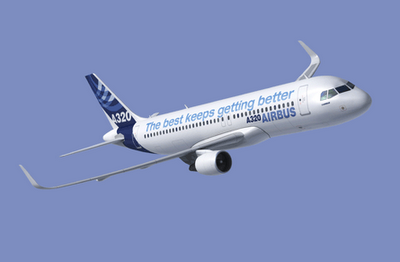
\includegraphics[width=0.49\linewidth]{Figures/Airbus_A320_sharklets.png}}
    \subfigure[Bombardier CRJ200]{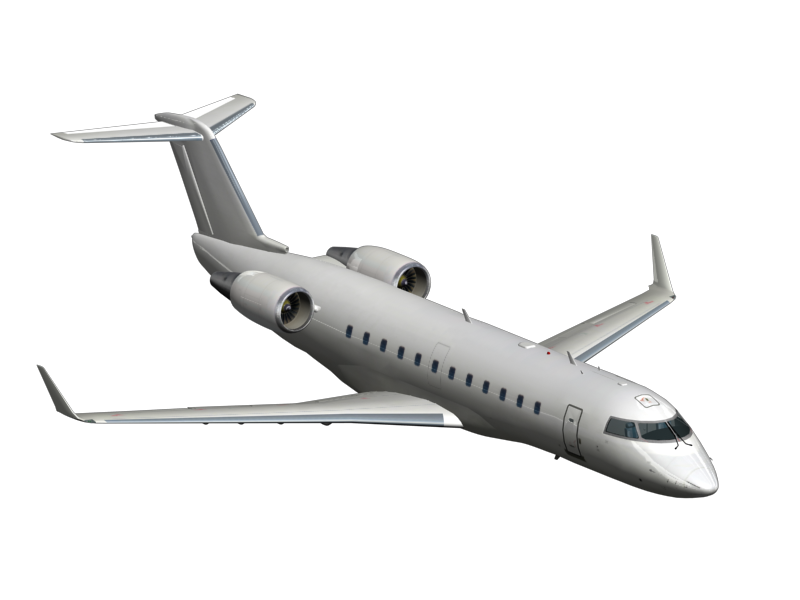
\includegraphics[width=0.49\linewidth]{Figures/Bombardier_CRJ200.png}}
  \end{subfigmatrix}
  \caption{Some aircrafts.}
  \label{fig:aircrafts}
\end{figure}

Make reference to Figures \ref{fig:airbus1} and \ref{fig:aircrafts}.

By default, the supported file types are {\it .png,.pdf,.jpg,.mps,.jpeg,.PNG,.PDF,.JPG,.JPEG}.

See \url{http://mactex-wiki.tug.org/wiki/index.php/Graphics_inclusion} for adding support to other extensions.


% ----------------------------------------------------------------------
\subsubsection{Drawings}
\label{subsection:drawings}

Insert your subsection material and for instance a few drawings...

The schematic illustrated in Fig.~\ref{fig:algorithm} can represent some sort of algorithm.

\begin{figure}[!htb]
  \centering
  \scriptsize
%  \footnotesize 
%  \small
  \setlength{\unitlength}{0.9cm}
  \begin{picture}(8.5,6)
    \linethickness{0.3mm}

    \put(3,6){\vector(0,-1){1}}
    \put(3.5,5.4){$\bf \alpha$}
    \put(3,4.5){\oval(6,1){}}
    %\put(0,4){\framebox(6,1){}}
    \put(0.3,4.4){Grid Generation: \quad ${\bf x} = {\bf x}\left({\bf \alpha}\right)$}

    \put(3,4){\vector(0,-1){1}}
    \put(3.5,3.4){$\bf x$}
    \put(3,2.5){\oval(6,1){}}
    %\put(0,2){\framebox(6,1){}}
    \put(0.3,2.4){Flow Solver: \quad ${\cal R}\left({\bf x},{\bf q}\left({\bf x}\right)\right) = 0$}

    \put(6.0,2.5){\vector(1,0){1}}
    \put(6.4,3){$Y_1$}

    \put(3,2){\vector(0,-1){1}}
    \put(3.5,1.4){$\bf q$}
    \put(3,0.5){\oval(6,1){}}
    %\put(0,0){\framebox(6,1){}}
    \put(0.3,0.4){Structural Solver: \quad ${\cal M}\left({\bf x},{\bf q}\left({\bf x}\right)\right) = 0$}

    \put(6.0,0.5){\vector(1,0){1}}
    \put(6.4,1){$Y_2$}

    %\put(7.8,2.5){\oval(1.6,5){}}
    \put(7.0,0){\framebox(1.6,5){}}
    \put(7.1,2.5){Optimizer}
    \put(7.8,5){\line(0,1){1}}
    \put(7.8,6){\line(-1,0){4.8}}
  \end{picture}
  \caption{Schematic of some algorithm.}
  \label{fig:algorithm}
\end{figure}


% ----------------------------------------------------------------------
\subsection{Equations}
\label{subsection:equations}

Equations can be inserted in different ways.

The simplest way is in a separate line like this

\begin{equation}
  \frac{{\rm d} q_{ijk}}{{\rm d} t} + {\cal R}_{ijk}({\bf q}) = 0 \,.
\label{eq:ode}
\end{equation}

If the equation is to be embedded in the text. One can do it like this ${\partial {\cal R}}/{\partial {\bf q}}=0$.

It may also be split in different lines like this

\begin{eqnarray}
  {\rm Minimize}   && Y({\bf \alpha},{\bf q}({\bf \alpha}))            \nonumber           \\
  {\rm w.r.t.}     && {\bf \alpha} \,,                                 \label{eq:minimize} \\
  {\rm subject~to} && {\cal R}({\bf \alpha},{\bf q}({\bf \alpha})) = 0 \nonumber           \\
                   &&       C ({\bf \alpha},{\bf q}({\bf \alpha})) = 0 \,. \nonumber
\end{eqnarray}

It is also possible to use subequations. Equations~\ref{eq:continuity}, \ref{eq:momentum} and \ref{eq:energy} form the Naver--Stokes equations~\ref{eq:NavierStokes}.

\begin{subequations}
    \begin{equation}
    \frac{\partial \rho}{\partial t} + \frac{\partial}{\partial x_j}\left( \rho u_j \right) = 0 \,,
    \label{eq:continuity}
    \end{equation}
    \begin{equation}
    \frac{\partial}{\partial t}\left( \rho u_i \right) + \frac{\partial}{\partial x_j} \left( \rho u_i u_j + p \delta_{ij} - \tau_{ji} \right) = 0, \quad i=1,2,3 \,,
    \label{eq:momentum}
    \end{equation}
    \begin{equation}
        \frac{\partial}{\partial t}\left( \rho E \right) + \frac{\partial}{\partial x_j} \left( \rho E u_j + p u_j - u_i \tau_{ij} + q_j \right) = 0 \,.
    \label{eq:energy}
    \end{equation}
\label{eq:NavierStokes}%
\end{subequations}


% ----------------------------------------------------------------------
\subsection{Tables}
\label{section:tables}

Insert your subsection material and for instance a few tables...

Make sure all tables presented are referenced in the text!

Follow some guidelines when making tables:

\begin{itemize}
  \item Avoid vertical lines
  \item Avoid “boxing up” cells, usually 3 horizontal lines are enough: above, below, and after heading
  \item Avoid double horizontal lines
  \item Add enough space between rows
\end{itemize}

\begin{table}[!htb]
  \renewcommand{\arraystretch}{1.2} % more space between rows
  \centering
  \begin{tabular}{lccc}
    \toprule
    Model           & $C_L$ & $C_D$ & $C_{M y}$ \\
    \midrule
    Euler           & 0.083 & 0.021 & -0.110    \\
    Navier--Stokes  & 0.078 & 0.023 & -0.101    \\
    \bottomrule
  \end{tabular}
  \caption[Table caption shown in TOC.]{Table caption.}
  \label{tab:aeroCoeff}
\end{table}

Make reference to Table \ref{tab:aeroCoeff}.

Tables \ref{tab:memory} and \ref{tab:multipleColumns} are examples of tables with merging columns:

\begin{table}[!htb]
  \renewcommand{\arraystretch}{1.2} % more space between rows
  \centering
  \begin{tabular}[]{lrr}
    \toprule
                & \multicolumn{2}{c}{\underline{Virtual memory [MB]}} \\
                & Euler       & Navier--Stokes \\
    \midrule
      Wing only &  1,000      &    2,000       \\
      Aircraft  &  5,000      &   10,000       \\
      (ratio)   & $5.0\times$ & $5.0\times$    \\
    \bottomrule
  \end{tabular}
  \caption{Memory usage comparison (in MB).}
  \label{tab:memory}
\end{table}

\begin{table}[!htb]
  \centering
  \renewcommand{\arraystretch}{1.2} % more space between rows
  \begin{tabular}{@{}rrrrcrrr@{}} % remove space to the vertical edges @{}...@{}
    \toprule
      & \multicolumn{3}{c}{$w = 2$} & \phantom{abc} & \multicolumn{3}{c}{$w = 4$} \\
    \cmidrule{2-4}
    \cmidrule{6-8}
      & $t=0$ & $t=1$ & $t=2$ && $t=0$ & $t=1$ & $t=2$ \\
    \midrule
      $dir=1$
      \\
      $c$ &  0.07 &  0.16 &  0.29 &&  0.36 &  0.71 &   3.18 \\
      $c$ & -0.86 & 50.04 &  5.93 && -9.07 & 29.09 &  46.21 \\
      $c$ & 14.27 &-50.96 &-14.27 && 12.22 &-63.54 &-381.09 \\
      $dir=0$
      \\
      $c$ &  0.03 &  1.24 &  0.21 &&  0.35 & -0.27 &  2.14 \\
      $c$ &-17.90 &-37.11 &  8.85 &&-30.73 & -9.59 & -3.00 \\
      $c$ &105.55 & 23.11 &-94.73 &&100.24 & 41.27 &-25.73 \\
    \bottomrule
  \end{tabular}
  \caption{Another table caption.}
  \label{tab:multipleColumns}
\end{table}

An example with merging rows can be seen in Tab.\ref{tab:multipleRows}.

\begin{table}[!htb]
  \renewcommand{\arraystretch}{1.2} % more space between rows
  \centering
  \begin{tabular}{ccccc}
    \toprule
      \multirow{2}{*}{ABC} & \multicolumn{4}{c}{header} \\
      \cmidrule{2-5} & 1.1 & 2.2 & 3.3 & 4.4 \\
    \midrule
      \multirow{2}{*}{IJK} & \multicolumn{2}{c}{\multirow{2}{*}{group}} & 0.5 & 0.6 \\
      \cmidrule{4-5}       & \multicolumn{2}{c}{}                       & 0.7 & 1.2 \\
    \bottomrule
  \end{tabular}
  \caption{Yet another table caption.}
  \label{tab:multipleRows}
\end{table}

If the table has too many columns, it can be scaled to fit the text widht, as in Tab.\ref{tab:scale}.
\begin{table}[!htb]
  \renewcommand{\arraystretch}{1.2} % more space between rows
  \centering
  \resizebox*{\textwidth}{!}{%
    \begin{tabular}[]{lcccccccccc}
      \toprule
        Variable &  a  &  b  &  c  &  d  &  e  &  f  &  g  &  h  &  i  &  j  \\
      \midrule
        Test 1   &  10,000 &  20,000 &  30,000 &  40,000 &  50,000 &  60,000 &  70,000 &  80,000 &  90,000 & 100,000 \\
        Test 2   &  20,000 &  40,000 &  60,000 &  80,000 & 100,000 & 120,000 & 140,000 & 160,000 & 180,000 & 200,000 \\
      \bottomrule
    \end{tabular}
  }%
  \caption{Very wide table.}
  \label{tab:scale}%
\end{table}


% ----------------------------------------------------------------------
\subsection{Mixing}
\label{section:mixing}

If necessary, a figure and a table can be put side-by-side as in Fig.\ref{fig:side_by_side}

\begin{figure}[!htb]
  \begin{minipage}[b]{0.60\linewidth}
    \centering
    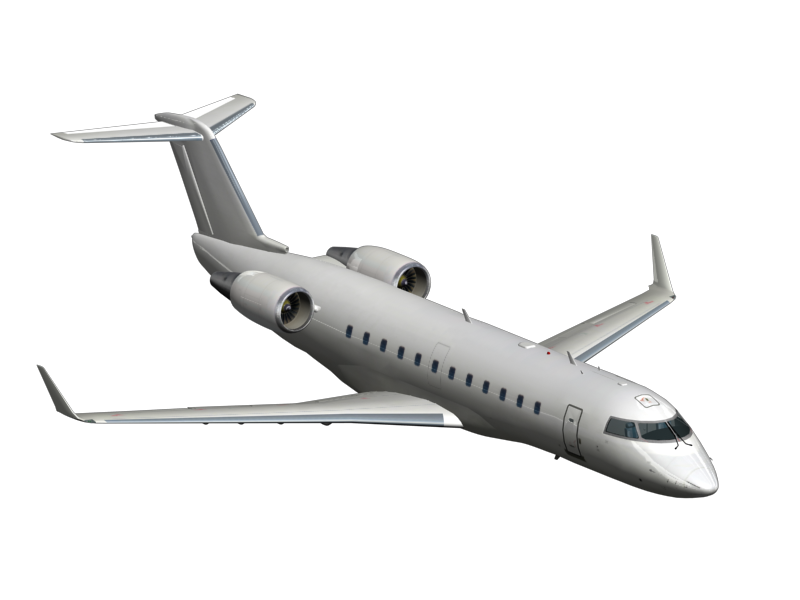
\includegraphics[width=\linewidth]{Figures/Bombardier_CRJ200}
  \end{minipage}%
  \begin{minipage}[b]{0.30\linewidth}
    \centering
    \begin{tabular}[b]{lll}
      \toprule
        \multicolumn{3}{c}{Legend} \\
      \midrule
        A & B & C \\
        0 & 0 & 0 \\
        0 & 1 & 0 \\
        1 & 0 & 0 \\
        1 & 1 & 1 \\
      \bottomrule
    \end{tabular}
    \vspace{5em}
  \end{minipage}
\caption{Figure and table side-by-side.}
\label{fig:side_by_side}
\end{figure}

 % file "Thesis_Results.tex"
\cleardoublepage

%%%%%%%%%%%%%%%%%%%%%%%%%%%%%%%%%%%%%%%%%%%%%%%%%%%%%%%%%%%%%%%%%%%%%%%%
%                                                                      %
%     File: Thesis_Conclusions.tex                                     %
%     Tex Master: Thesis.tex                                           %
%                                                                      %
%     Author: Andre C. Marta                                           %
%     Last modified :  2 Jul 2015                                      %
%                                                                      %
%%%%%%%%%%%%%%%%%%%%%%%%%%%%%%%%%%%%%%%%%%%%%%%%%%%%%%%%%%%%%%%%%%%%%%%%

\chapter{Conclusions and Future Work}
\label{chapter:conclusions}

\section{Conclusions}

The lack of security in \gls{iot} is a serious issue that can lead to a high monetary costs,
especially when botnets infect the devices. Recent
attacks clearly show that serious damage can be caused \cite{sec17ant94:online}. An old saying attributed to the
\gls{nsa} states that "Attacks always get better; they never get worse".
Combined with the fact that the number of \gls{iot} devices is growing at a high
pace, without any major improvements to their security, makes it clear
that it is fundamental for this issue to be addressed.

\gls{tls} is one of the most used communication security protocols in the world. It offers the
security services of authentication, confidentiality, privacy, integrity, replay
protection and perfect forward secrecy. It is not a requirement to use all of
those services for every TLS connection. The protocol is similar to
a framework, in the sense that you can enable some of the security
services on a per-connection basis.

While \gls{tls} does have many configurations, not all of them can be used with the \gls{iot},
due to the constrained nature of the devices. In many cases it is necessary to make security/cost
trade-offs. In order to be able to make them, it is important to know the costs of each security
service. Current work offers no such information. Thus, a software developer wishing to use \gls{tls}
for connection security in a constrained environment does not have a reference to go to.

In our work, we decomposed \gls{tls} into individual parts and evaluated the cost of each security service.
We have evaluated the cost of every \gls{tls} configuration available in \textit{mbedTLS 2.7.0} and the underlying
algorithms. The herein presented results can be used to make informed decisions about the security/cost trade-offs,
specific to the environment.

First, we did a thorough analysis of \gls{tls}, by analyzing the number of estimated CPU cycles obtained with \textit{callgrind}.
After that, we showed that the estimates are close to the real values, by comparing them to the time metrics obtained directly from
the processor's registers. The results presented here were obtained on a powerful, modern-day computer. Despite that, they are still
relevant when considering the costs on constrained \gls{iot} devices. While on a different device, the absolute cost 
numbers will be different, they would still maintain a similar proportion one to another and follow a similar trend.
Moreover, the developed tooling can be used to obtain profiling results on any machine, thus giving device-specific 
cost information. The formula used to obtain the CPU cycle count estimate can also be changed to one's needs.

\section{Future Work}

In our work we obtained and analyzed a large number of metrics obtained with \textit{callgrind}. While \textit{callgrind}
provides only an estiamtes of the CPU cycles used, we later showed  that they reflect real values by comparing them with the
time results obtained with \gls{papi}. However, it is important to remember that those mertics were obtained on a general-purpose
computer. While we fixed the CPU frequency and disabled some hardware optimizations, the environment on an \gls{iot} device is still
expected to be very different, due factors such as a lower clock frequency, memory and cache size. Thus, it would be interesting to 
measure time on an gls{iot} device, since the results will differ.

Another characteristic of numerous \gls{iot} devices is limited power (\textit{e.g.} using battery as a power source). 
Thus, it would be interesting analyze the cost of \gls{tls} in terms of power usage. This would also allow to reach 
interesting conclusions, such as: \textit{Using the TLS configuration X would reduce the device's battery life by Y days}. % file "Thesis_Conclusions.tex"
\cleardoublepage

% ----------------------------------------------------------------------
%  Bibliography
% ----------------------------------------------------------------------

% Add entry in the table of contents as chapter
\phantomsection
\addcontentsline{toc}{chapter}{\bibname}

% Include all references in .bib file, even non-cited ones...
%\nocite{*} % this should be used carefully because it is not correct!

% Produces the bibliography section when processed by BibTeX
%
% Bibliography style
% > entries ordered alphabetically
%\bibliographystyle{plain}
% > unsorted with entries appearing in the order in which the citations appear.
%\bibliographystyle{unsrt}
% > entries ordered alphabetically, with first names and names of journals and months abbreviated
%\bibliographystyle{abbrv}
% > entries ordered alphabetically, with reference markers based on authors' initials and publication year
%\bibliographystyle{alpha}
%
% Replacement bibliography styles provided by 'natbib' package
% (plainnat.bst, abbrvnat.bst, unsrtnat.bst )
% > entries ordered alphabetically
%\bibliographystyle{plainnat}
% > unsorted with entries appearing in the order in which the citations appear.
%\bibliographystyle{unsrtnat}
% > entries ordered alphabetically, with first names and names of journals and months abbreviated
%\bibliographystyle{abbrvnat} % <<<<< SELECT IF USING REFERENCES BY AUTHOR/YEAR
% > entries ordered alphabetically, with reference markers based on authors' initials and publication year
%\bibliographystyle{alpha}
%
% Custom bibliography style adapted from 'natbib' package
%   (based on http://tex.stackexchange.com/questions/5053/is-it-possible-to-get-unsrt-abbrv-bibliography)
%   (unsrtnat.bst + abbrvnat.bst -> abbrvunsrtnat.bst)
%   (original files copied from:
%   http://tug.ctan.org/macros/latex/contrib/natbib/abbrvnat.bst
%   http://tug.ctan.org/macros/latex/contrib/natbib/unsrtnat.bst
% > unsorted with entries appearing in the order in which the citations appear, with first names and names of journals and months abbreviated.
\bibliographystyle{abbrvunsrtnat} % <<<<< SELECT IF USING REFERENCES BY NUMBER (CITATION ORDER)

% External bibliography database file in the BibTeX format
\bibliography{tls_for_iot,papers} % file "Thesis_bib_DB.bib"

\cleardoublepage

% ----------------------------------------------------------------------
%  Appendix (optional)
%
%  CAUTION: 1) the main document (up to the conclusions) shall not exceed 80 pages
%           2) the document shall not exceed a total of 100 pages (per IST regulations)
% ----------------------------------------------------------------------
\appendix

% add page number prefix according to apendix chapter (optional)
%\renewcommand{\thepage}{\thechapter.\arabic{page}}

% re-set arabic numbering (A.1,A.2,...) (optional, use only if chapter prefix is added)
%\setcounter{page}{1}

%%%%%%%%%%%%%%%%%%%%%%%%%%%%%%%%%%%%%%%%%%%%%%%%%%%%%%%%%%%%%%%%%%%%%%%%
%                                                                      %
%     File: Thesis_Appendix_A.tex                                      %
%     Tex Master: Thesis.tex                                           %
%                                                                      %
%     Author: Andre C. Marta                                           %
%     Last modified :  2 Jul 2015                                      %
%                                                                      %
%%%%%%%%%%%%%%%%%%%%%%%%%%%%%%%%%%%%%%%%%%%%%%%%%%%%%%%%%%%%%%%%%%%%%%%%

\chapter{Appendix A}

\begin{table}[]
	\resizebox{\textwidth}{!}{
	\begin{tabular}{|l|l|l|l|l|}
	\hline
	\backslashbox{Security\\Level}{Operation}                  & \textbf{RSA Sign}    & \textbf{RSA Verify} & \textbf{ECDSA Sign} & \textbf{ECDSA Verify} \\ \hline
	\textbf{low}       & 20559190 (117075)    & 398584 (198)        & 14497591 (49045)    & 26839273 (50816)      \\ \hline
	\textbf{normal}    & 75738802 (317047)    & 1117868 (748)       & 29512991 (95776)    & 56260702 (162365)     \\ \hline
	\textbf{high}      & 317087210 (716961)   & 3295296 (254)       & 49150396 (82047)     & 94077150 (130275)     \\ \hline
	\textbf{very high} & 1700652764 (2283718) & 13436728 (702)      & 59732056 (441815)   & 114744021 (843861)    \\ \hline
	\end{tabular}}
	\centering \caption{\label{table:rsa-costs-all-sls} RSA and ECDSA signature creation and verification costs in number of CPU cycles. Numbers in parenthesis is the standard deviation} \end{table}
  
  \begin{table}[]
	\begin{tabular}{|l|l|l|}
	\hline
	\backslashbox{Security\\Level}{Operation}                   & \textbf{RSA Total} & \textbf{ECDSA Total} \\ \hline
	\textbf{low}       & 20957774           & 41336864             \\ \hline
	\textbf{normal}    & 76856670           & 85773693             \\ \hline
	\textbf{high}      & 320382506          & 143227546            \\ \hline
	\textbf{very high} & 1714089492         & 174476077            \\ \hline
	\end{tabular}
	\centering \caption{\label{table:rsa-costs-all-sls-total} RSA and ECDSA costs of signature creation + signature verification in number of CPU cycles}
  \end{table}
  
  \begin{table}[]
	\begin{tabular}{|l|l|l|l|}
	\hline
   \backslashbox{Security\\Level}{Opeation}                    & \textbf{RSA Sign} & \textbf{RSA Verify} & \textbf{RSA Total} \\ \hline
	\textbf{low}       & -                 & -                   & -                  \\ \hline
	\textbf{normal}    & 55179612          & 719284              & 55898896           \\ \hline
	\textbf{high}      & 241348408         & 2177428             & 243525836          \\ \hline
	\textbf{very high} & 1383565554        & 10141432            & 1393706986         \\ \hline
	\end{tabular}
	\centering \caption{\label{table:rsa-absolute-cost-increase} Absolute increase of RSA operation costs from previous security level in number of CPU cycles}
	\end{table}
  
  \begin{table}[]
  \begin{tabular}{|l|l|l|l|}
  \hline
   \backslashbox{Security\\Level}{Opeation}                  & \textbf{ECDSA Sign} & \textbf{ECDSA Verify} & \textbf{ECDSA Total} \\ \hline
  \textbf{low}       & -                   & -                     & -                    \\ \hline
  \textbf{normal}    & 15015400            & 29421429              & 44436829             \\ \hline
  \textbf{high}      & 19637405            & 37816448              & 57453853             \\ \hline
  \textbf{very high} & 10581660            & 20666871              & 31248531             \\ \hline
  \end{tabular}
  \centering \caption{\label{table:ecdsa-absolute-cost-increase} Absolute increase of ECDSA operations cost from previous security level in number of CPU cycles}
  \end{table}
  
  \begin{table}[]
	\begin{tabular}{|l|l|l|l|l|}
	\hline
	 \backslashbox{Key\\Exchange}{Security\\Level}                     & \textbf{low} & \textbf{normal} & \textbf{high} & \textbf{very high} \\ \hline
	\textbf{PSK}         & 0            & 0               & 0             & 0                  \\ \hline
	\textbf{RSA}         & 654077       & 2622235         & 5285561       & 16398134           \\ \hline
	\textbf{RSA-PSK}     & 654077       & 2622235         & 5285561       & 16398134           \\ \hline
	\textbf{ECDH-RSA}    & 1117868      & 1117868         & 1117868       & 1117868           \\ \hline
	\textbf{ECDH-ECDSA}  & 56260702     & 56260702        & 56260702      & 56260702          \\ \hline
	\textbf{ECDHE-PSK}   & 0            & 0               & 0             & 0                  \\ \hline
	\textbf{ECDHE-RSA}   & 1516452       & 2235736         & 4413164       & 14554596           \\ \hline
	\textbf{ECDHE-ECDSA} & 83099975     & 112521404       & 150337852     & 171004723          \\ \hline
	\textbf{DHE-PSK}     & 0            & 0               & 0             & 0                  \\ \hline
	\textbf{DHE-RSA}     & 1516452       & 2235736         & 4413164       & 14554596           \\ \hline
	\end{tabular}
	\centering \caption{\label{table:tls-auth-cost-client} Client authentication costs for all ciphersuites and security levels in number of CPU cycles}
	\end{table}
  
  \begin{table}[]
  \begin{tabular}{|l|l|l|l|l|}
  \hline
   \backslashbox{Key\\Exchange}{Security\\Level}                     & \textbf{low} & \textbf{normal} & \textbf{high} & \textbf{very high} \\ \hline
  \textbf{PSK}         & 0            & 0               & 0             & 0                  \\ \hline
  \textbf{RSA}         & 20362831     & 75129504        & 314975365     & 1691976601         \\ \hline
  \textbf{RSA-PSK}     & 20362831     & 75129504        & 314975365     & 1691976601         \\ \hline
  \textbf{ECDH-RSA}    & 0            & 0               & 0             & 0                  \\ \hline
  \textbf{ECDH-ECDSA}  & 0            & 0               & 0             & 0                  \\ \hline
  \textbf{ECDHE-PSK}   & 0            & 0               & 0             & 0                  \\ \hline
  \textbf{ECDHE-RSA}   & 20559190     & 75738802        & 317087210     & 1700652764         \\ \hline
  \textbf{ECDHE-ECDSA} & 14497591     & 29512991        & 49150396      & 59732056           \\ \hline
  \textbf{DHE-PSK}     & 0            & 0               & 0             & 0                  \\ \hline
  \textbf{DHE-RSA}     & 20559190     & 75738802        & 317087210     & 1700652764         \\ \hline
  \end{tabular}
	\centering \caption{\label{table:tls-auth-cost-server} Server authentication costs for all ciphersuites and security levels in number of CPU cycles}
  \end{table}
  
  \begin{table}[]
  \resizebox{\textwidth}{!}{
  \begin{tabular}{|l|l|l|l|l|}
  \hline
   \backslashbox{Security\\Level}{Opeation}                   & \textbf{ECDH Gen Keypair} & \textbf{ECDH Gen Secret} & \textbf{DH Gen Keypair} & \textbf{DH Gen Secret} \\ \hline
  \textbf{low}       & 12942518 (33356)          & 12462677 (55222)         & 10455300 (31005)        & 10279378 (27044)       \\ \hline
  \textbf{normal}    & 27483912 (94940)          & 26958612 (137745)        & 67136033 (108793)       & 66712994 (107669)      \\ \hline
  \textbf{high}      & 45900358 (65731)          & 44331330 (100040)        & 474938146 (490496)      & 473634908 (493588)     \\ \hline
  \textbf{very high} & 54449740 (487567)         & 53531554 (776984)        & 3592631108 (2792006)    & 3586324217 (2791154)   \\ \hline
  \end{tabular}}
  \centering \caption{\label{table:ecdh-dh-costs-all-sls} ECDH and DH costs for all security levels in number of CPU cycles. Numbers in parenthesis are the standard deviation.}
  \end{table}
  
  \begin{table}[]
  \begin{tabular}{|l|l|l|}
  \hline
   \backslashbox{Security\\Level}{Operation}                   & \textbf{ECDH Total} & \textbf{DH Total} \\ \hline
  \textbf{low}       & 25405195            & 20734678          \\ \hline
  \textbf{normal}    & 54442524            & 133849027         \\ \hline
  \textbf{high}      & 90231688            & 948573054         \\ \hline
  \textbf{very high} & 90231688            & 7178955325        \\ \hline
  \end{tabular}
  \centering \caption{\label{table:ecdh-dh-costs-total-all-sls} ECDH and DH costs of the sum of keypair and shared secret generation in number of CPU cycles}
  \end{table}
  
  \begin{table}[]
  \begin{tabular}{|l|l|l|l|}
  \hline
   \backslashbox{Security\\Level}{Operation}                   & \textbf{ECDH Gen Keypair} & \textbf{ECDH Gen Shared} & \textbf{ECDH Total} \\ \hline
  \textbf{low}       & -                         & -                        & -                   \\ \hline
  \textbf{normal}    & 14541394                  & 14495935                 & 29037329            \\ \hline
  \textbf{high}      & 18416446                  & 17372718                 & 35789164            \\ \hline
  \textbf{very high} & 8549382                   & 9200224                  & 17749606            \\ \hline
  \end{tabular}
  \centering \caption{\label{table:ecdh-absolute-cost-increase} Absolute increase of ECDH operation costs from previous security level in number of CPU cycles}
  \end{table}
  
  \begin{table}[]
	  \begin{tabular}{|l|l|l|l|}
	  \hline
	   \backslashbox{Security\\ Level}{Operation}                   & \textbf{DH Gen Keypair} & \textbf{DH Gen Shared} & \textbf{DH Total} \\ \hline
	  \textbf{low}       & -                       & -                      & -                 \\ \hline
	  \textbf{normal}    & 56680733                & 56433616               & 113114349         \\ \hline
	  \textbf{high}      & 407802113               & 406921914              & 814724027         \\ \hline
	  \textbf{very high} & 3117692962              & 3112689309             & 6230382271        \\ \hline
	  \end{tabular}
	  \centering \caption{\label{table:dh-absolute-cost-increase} Absolute increase of DH operation costs from previous security level in number of CPU cycles}
  \end{table}
  
  \begin{table}[]
  \begin{tabular}{|l|l|l|l|l|}
  \hline
   \backslashbox{Key\\Exchange}{Security\\Level}                                           & \textbf{low}                    & \textbf{normal}                 & \textbf{high}                   & \textbf{very high}               \\ \hline
  \textbf{PSK}                               & 0                               & 0                               & 0                               & 0                                \\ \hline
  \textbf{RSA-PSK}                           & 0                               & 0                               & 0                               & 0                                \\ \hline
  \textbf{RSA}                               & 0                               & 0                               & 0                               & 0                                \\ \hline
  \rowcolor[HTML]{9B9B9B}
  {\color[HTML]{333333} \textbf{ECDH-RSA}}   & {\color[HTML]{333333} 25405195} & {\color[HTML]{333333} 54442524} & {\color[HTML]{333333} 90231688} & {\color[HTML]{333333} 107981294} \\ \hline
  \rowcolor[HTML]{9B9B9B}
  {\color[HTML]{333333} \textbf{ECDH-ECDSA}} & {\color[HTML]{333333} 25405195} & {\color[HTML]{333333} 54442524} & {\color[HTML]{333333} 90231688} & {\color[HTML]{333333} 107981294} \\ \hline
  \textbf{ECDHE-PSK}                         & 25405195                        & 54442524                        & 90231688                        & 107981294                        \\ \hline
  \textbf{ECDHE-RSA}                         & 25405195                        & 54442524                        & 90231688                        & 107981294                        \\ \hline
  \textbf{ECDHE-ECDSA}                       & 25405195                        & 54442524                        & 90231688                        & 107981294                        \\ \hline
  \textbf{DHE-PSK}                           & 20734678                        & 133849027                       & 948573054                        & 7178955325                        \\ \hline
  \textbf{DHE-RSA}                           & 25405195                        & 133849027                        & 948573054                        & 7178955325                        \\ \hline
  \end{tabular}
  \centering \caption{\label{table:pfs-cost-client} \gls{pfs} and \textit{ECDH} key exchange cost for the client in number of CPU cycles}
  \end{table}
  
  \begin{table}[]
  \begin{tabular}{|l|l|l|l|l|}
  \hline
   \backslashbox{Key\\Exchange}{Security\\Level}                                           & \textbf{low}                    & \textbf{normal}                 & \textbf{high}                   & \textbf{very high}              \\ \hline
  \textbf{PSK}                               & 0                               & 0                               & 0                               & 0                               \\ \hline
  \textbf{RSA-PSK}                           & 0                               & 0                               & 0                               & 0                               \\ \hline
  \textbf{RSA}                               & 0                               & 0                               & 0                               & 0                               \\ \hline
  \rowcolor[HTML]{9B9B9B}
  {\color[HTML]{333333} \textbf{ECDH-RSA}}   & {\color[HTML]{333333} 12462677} & {\color[HTML]{333333} 26958612} & {\color[HTML]{333333} 44331330} & {\color[HTML]{333333} 53531554} \\ \hline
  \rowcolor[HTML]{9B9B9B}
  {\color[HTML]{333333} \textbf{ECDH-ECDSA}} & {\color[HTML]{333333} 12462677} & {\color[HTML]{333333} 26958612} & {\color[HTML]{333333} 44331330} & {\color[HTML]{333333} 53531554} \\ \hline
  \textbf{ECDHE-PSK}                         & 25405195                        & 54442524                        & 90231688                        & 107981294                       \\ \hline
  \textbf{ECDHE-RSA}                         & 25405195                        & 54442524                        & 90231688                        & 107981294                       \\ \hline
  \textbf{ECDHE-ECDSA}                       & 25405195                        & 54442524                        & 90231688                        & 107981294                       \\ \hline
  \textbf{DHE-PSK}                           & 20734678                        & 133849027                       & 948573054                        & 7178955325                       \\ \hline
  \textbf{DHE-RSA}                           & 20734678                        & 133849027                       & 948573054                        & 7178955325                       \\ \hline
  \end{tabular}
  \centering \caption{\label{table:pfs-cost-server} \gls{pfs} and \textit{ECDH} key exchange cost for the server in number of CPU cycles}
  \end{table}
  
  \begin{table}[]
	\resizebox{\textwidth}{!}{
	\begin{tabular}{|l|l|l|l|l|}
	\hline
	 \backslashbox{Key\\Exchange}{Security\\Level}                     & \textbf{low}      & \textbf{normal}    & \textbf{high}      & \textbf{very high}   \\ \hline
	\textbf{PSK}         & 1354543 (51058)   & 1353865 (51289)    & 1355005 (51004)    & 1354829 (51043)      \\ \hline
	\textbf{RSA-PSK}     & 3536763 (71446)   & 4543238 (76038)    & 7293473 (84814)    & 18578392 (103341)    \\ \hline
	\textbf{RSA}         & 3556430 (59010)   & 4558935 (68078)    & 7309587 (71844)    & 18608492 (82623)     \\ \hline
	\textbf{ECDH-RSA}    & 28433250 (97731)  & 57412269 (122298)  & 93325335 (102107)  & 111532116 (623350)   \\ \hline
	\textbf{ECDH-ECDSA}  & 83731926 (78435)  & 112585306 (128327) & 148415289 (126285) & 166815336 (554471)   \\ \hline
	\textbf{ECDHE-PSK}   & 26819362 (68991)  & 55805138 (138561)  & 91713096 (142807)  & 109203285 (813689)   \\ \hline
	\textbf{ECDHE-RSA}   & 28862986 (105477) & 58608367 (214574)  & 96730901 (93708)   & 124773055 (696488)   \\ \hline
	\textbf{ECDHE-ECDSA} & 110524836 (93990) & 168954007 (267635) & 242501399 (149155) & 280626510 (1071418)  \\ \hline
	\textbf{DHE-PSK}     & 22189619 (55603)  & 135442518 (309751) & 950212732 (787892) & 7181764421 (5195398) \\ \hline
	\textbf{DHE-RSA}     & 24250886 (94421)  & 138197524 (198704) & 955840114 (861069) & 7196088947 (6405987) \\ \hline
	\end{tabular}}
	\centering \caption{\label{table:client-hs-cost-all-sls} Handshake costs for the client in number of CPU cycles. Numbers in parenthesis are the standard deviation}
	\end{table}
  
	\begin{table}[]
		\resizebox{\textwidth}{!}{
  \begin{tabular}{|l|l|l|l|l|}
  \hline
   \backslashbox{Key\\Exchange}{Security\\Level}                     & \textbf{low}      & \textbf{normal}    & \textbf{high}       & \textbf{very high}   \\ \hline
  \textbf{PSK}         & 1380956 (50888)   & 1382849 (50737)    & 1381497 (50891)     & 1382002 (50903)      \\ \hline
  \textbf{RSA-PSK}     & 22515609 (111975) & 77368868 (275574)  & 317389619 (662953)  & 1694178055 (2427763) \\ \hline
  \textbf{RSA}         & 22456180 (121140) & 77260738 (239418)  & 317196961 (698637)  & 1694747500 (1705523) \\ \hline
  \textbf{ECDH-RSA}    & 14534087 (49806)  & 29154666 (127699)  & 46480720 (107771)   & 55636527 (576001)    \\ \hline
  \textbf{ECDH-ECDSA}  & 14521154 (58001)  & 29094320 (111114)  & 46390603 (132250)   & 55927921 (688074)    \\ \hline
  \textbf{ECDHE-PSK}   & 26869449 (110405) & 56020895 (147825)  & 91773474 (94656)    & 109500050 (905013)   \\ \hline
  \textbf{ECDHE-RSA}   & 48164890 (126885) & 132433386 (379327) & 409652623 (951326)  & 1810563620 (3011341) \\ \hline
  \textbf{ECDHE-ECDSA} & 41984222 (82371)  & 86096716 (192885)  & 141506181 (147013)  & 169996896 (1051307)  \\ \hline
  \textbf{DHE-PSK}     & 22308029 (76182)  & 135535409 (232955) & 950691653 (1289706) & 7181243788 (5402427) \\ \hline
  \textbf{DHE-RSA}     & 43602094 (154553) & 212251542 (364611) & 1268235354 (857921) & 8883866054 (5993186) \\ \hline
  \end{tabular}}
	\centering \centering \caption{\label{table:server-hs-cost-all-sls} Handshake costs for the server in number of CPU cycles. Numbers in parenthesis are the standard deviation}
  \end{table}
  
  
	  \begin{table}[]
		\begin{tabular}{|l|l|l|l|l|}
		\hline
		\backslashbox{Security\\Level}{Operation}                 & \textbf{RSA Sign} & \textbf{RSA Verify} & \textbf{ECDSA Sign} & \textbf{ECSDA Verify} \\ \hline
		\textbf{low}       & 11355 (138)       & 293 (5)             & 8487 (2010)         & 14219 (175)           \\ \hline
		\textbf{normal}    & 41672 (342)       & 747 (8)             & 16130 (441)         & 30750 (246)           \\ \hline
		\textbf{high}      & 176255 (997)      & 2096 (15)           & 26961 (221)         & 51457 (272)           \\ \hline
		\textbf{very high} & 939928 (3238)     & 7704 (33)           & 34246 (334)         & 65877 (549)           \\ \hline
		\end{tabular}
		\caption{RSA and ECDSA signature creation and verification costs in microseconds. Numbers in parenthesis is the standard deviation}
		\label{table:rsa-ecdsa-costs-papi}
		\end{table}
  
		\begin{table}[]
		  \begin{tabular}{|l|l|l|l|l|}
		  \hline
		   \backslashbox{Key\\Exchange}{Security\\Level}                    & \textbf{low} & \textbf{normal} & \textbf{high} & \textbf{very high} \\ \hline
		  \textbf{PSK}         & 0            & 0               & 0             & 0                  \\ \hline
		  \textbf{ECDHE-PSK}   & 0            & 0               & 0             & 0                  \\ \hline
		  \textbf{DHE-PSK}     & 0            & 0               & 0             & 0                  \\ \hline
		  \textbf{ECDH-RSA}    & 683 (9)       & 683 (6)          & 678 (11)       & 682 (6)             \\ \hline
		  \textbf{ECDHE-RSA}   & 1014 (120)    & 1446 (115)       & 2805 (122)     & 8406 (123)          \\ \hline
		  \textbf{DHE-RSA}     & 1000 (119)    & 1439 (103)       & 2798 (119)     & 8388 (126)          \\ \hline
		  \textbf{RSA}         & 1061 (14)     & 1712 (23)        & 3436 (25)      & 9806 (55)           \\ \hline
		  \textbf{RSA-PSK}     & 1060 (9)      & 1710 (22)        & 3438 (27)      & 9804 (51)           \\ \hline
		  \textbf{ECDH-ECDSA}  & 30722 (272)   & 30847 (243)      & 30631 (210)    & 30765 (363)         \\ \hline
		  \textbf{ECDHE-ECDSA} & 46368 (3693)  & 62989 (3636)     & 83322 (3383)   & 97615 (2980)        \\ \hline
		  \end{tabular}
		  \caption{Client authentication costs for all ciphersuites and security levels in microseconds}
		  \label{table:papi-cli-auth-cost}
		  \end{table}
  
		  \begin{table}[]
			\begin{tabular}{|l|l|l|l|l|}
			\hline
			\backslashbox{Key\\Exchange}{Security\\Level}                    & \textbf{low} & \textbf{normal} & \textbf{high} & \textbf{very high} \\ \hline
			\textbf{PSK}         & 0            & 0               & 0             & 0                  \\ \hline
			\textbf{ECDHE-PSK}   & 0            & 0               & 0             & 0                  \\ \hline
			\textbf{DHE-PSK}     & 0            & 0               & 0             & 0                  \\ \hline
			\textbf{ECDH-RSA}    & 0            & 0               & 0             & 0                  \\ \hline
			\textbf{ECDHE-RSA}   & 11342 (138)   & 41659 (342)      & 176241 (997)   & 939913 (3238)       \\ \hline
			\textbf{DHE-RSA}     & 11329 (135)   & 41689 (694)      & 176192 (1197)  & 939929 (3698)       \\ \hline
			\textbf{RSA}         & 11286 (178)   & 41403 (411)      & 175097 (1089)  & 936521 (3356)       \\ \hline
			\textbf{RSA-PSK}     & 11259 (156)   & 41372 (348)      & 175107 (1114)  & 935820 (3347)       \\ \hline
			\textbf{ECDH-ECDSA}  & 0            & 0               & 0             & 0                  \\ \hline
			\textbf{ECDHE-ECDSA} & 8474 (2008)   & 16117 (440)      & 26947 (221)    & 34231 (334)         \\ \hline
			\end{tabular}
			\caption{Server authentication costs for all ciphersuites and security levels in microseconds}
			\label{table:server-auth-costs-papi}
			\end{table}
  
			\begin{table}[]
				\resizebox{\textwidth}{!}{
			  \begin{tabular}{|l|l|l|l|l|}
			  \hline
			   \backslashbox{Security\\Level}{Operation}                  & \textbf{ECDH Gen Keypair} & \textbf{ECDH Gen Shared} & \textbf{DH Gen Keypair} & \textbf{DH Gen Shared} \\ \hline
			  \textbf{low}       & 6884 (45)                 & 6593 (67)                 & 6028 (127)               & 5878 (171)              \\ \hline
			  \textbf{normal}    & 15049 (158)                & 14693 (131)               & 37422 (325)              & 36969 (275)             \\ \hline
			  \textbf{high}      & 25139 (305)                & 24297 (187)               & 263498 (843)             & 262432 (927)            \\ \hline
			  \textbf{very high} & 31270 (342)                & 30830 (455)               & 1959755 (3784)           & 1955550 (4082)          \\ \hline
			  \end{tabular}}
			  \caption{ECDH  and  DH  costs  for  all  security  levels  in  microseconds.  Numbers  in parenthesis are the standard deviation}
			  \label{table:papi-ecd-dh-costs}
			  \end{table}
  
			  \begin{table}[]
				\begin{tabular}{|l|l|l|l|l|}
				\hline
				 \backslashbox{Key\\Exchange}{Security\\Level}                    & \textbf{low} & \textbf{normal} & \textbf{high} & \textbf{very high} \\ \hline
				\textbf{PSK}         & 1024 (97)    & 1038 (95)        & 1013 (82)      & 1028 (96)           \\ \hline
				\textbf{RSA-PSK}     & 2531 (121)    & 3204 (103)       & 4954 (125)     & 11388 (136)         \\ \hline
				\textbf{RSA}         & 2537 (132)    & 3202 (108)       & 4948 (124)     & 11387 (140)         \\ \hline
				\textbf{ECDH-RSA}    & 15709 (187)  & 31966 (309)      & 51570 (389)    & 64849 (538)         \\ \hline
				\textbf{ECDH-ECDSA}  & 45665 (384)   & 61924 (386)      & 81463 (385)    & 94748 (651)         \\ \hline
				\textbf{ECDHE-PSK}   & 14605 (148)  & 30893 (264)      & 50525 (438)    & 63219 (641)         \\ \hline
				\textbf{ECDHE-RSA}   & 16138 (344)  & 32831 (371)      & 53778 (397)    & 72269 (761)         \\ \hline
				\textbf{ECDHE-ECDSA} & 61255 (3776)  & 94156 (3729)     & 134140 (3479)  & 161190 (3168)       \\ \hline
				\textbf{DHE-PSK}     & 13086 (283)  & 75520 (426)      & 527114 (1356)  & 3916656 (6127)      \\ \hline
				\textbf{DHE-RSA}     & 14607(382)   & 77476 (521)      & 531919 (1841)  & 3930292 (6979)      \\ \hline
				\end{tabular}
				\caption{Handshake costs for the client in microseconds. Numbers in parenthesis are the standard deviation}
				\label{table:hs-costs-cli-papi}
				\end{table}
  
				\begin{table}[]
				  \begin{tabular}{|l|l|l|l|l|}
				  \hline
				   \backslashbox{Key\\Exchange}{Security\\Level}                    & \textbf{low} & \textbf{normal} & \textbf{high} & \textbf{very high} \\ \hline
				  \textbf{PSK}         & 1029 (90)     & 1048 (89)        & 1021 (76)      & 1033 (90)           \\ \hline
				  \textbf{RSA-PSK}     & 12668 (166)   & 42809 (355)      & 176543 (1118)  & 937388 (3348)       \\ \hline
				  \textbf{RSA}         & 12685 (188)   & 42828 (414)      & 176527 (1091)  & 938082 (3359)       \\ \hline
				  \textbf{ECDH-RSA}    & 8129 (180)    & 16187 (322)      & 26366 (2121)   & 32412 (483)         \\ \hline
				  \textbf{ECDH-ECDSA}  & 8137 (200)    & 16160 (170)      & 25842 (233)    & 32350 (473)         \\ \hline
				  \textbf{ECDHE-PSK}   & 14769 (256)   & 30919 (291)      & 50787 (321)    & 63563 (548)         \\ \hline
				  \textbf{ECDHE-RSA}   & 26628 (485)   & 73075 (591)      & 227665 (1194)  & 1004212 (3334)      \\ \hline
				  \textbf{ECDHE-ECDSA} & 24408 (4163)  & 48707 (3657)     & 79316 (3321)   & 98991 (2870)        \\ \hline
				  \textbf{DHE-PSK}     & 13139 (147)   & 75741 (423)      & 527735 (1390)  & 3925059 (9696)      \\ \hline
				  \textbf{DHE-RSA}     & 24964 (365)   & 117961 (1399)    & 704677 (1918)  & 4864588 (13183)     \\ \hline
				  \end{tabular}
				  \caption{Handshake costs for the server in microseconds. Numbers in parenthesis are the standard deviation}
				  \label{table:server-hs-costs-papi}
				  \end{table}
  
				  \begin{figure}
					\centering
					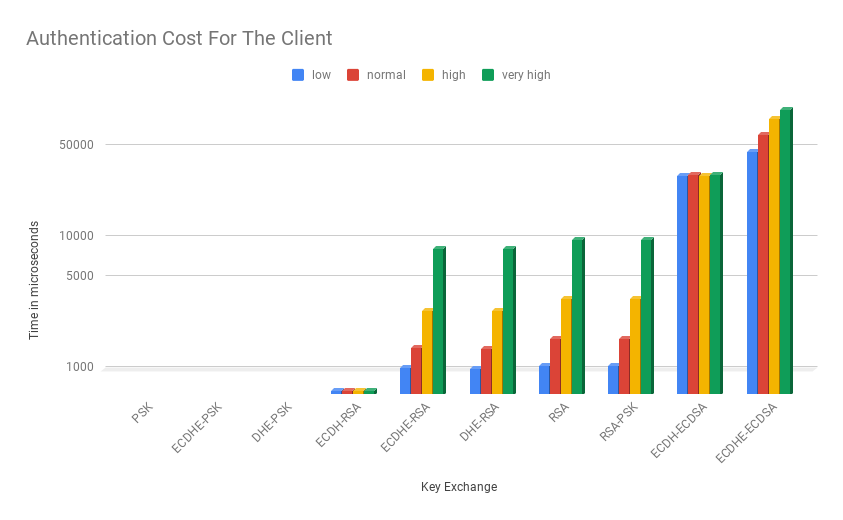
\includegraphics[width=1.0\textwidth]{img/papi-client-auth-cost.png}
					\centering \caption{Authentication cost for the client in microseconds (logarithmic scale)}
					\label{af:1}
				  \end{figure}
  
				  \begin{figure}
					\centering
					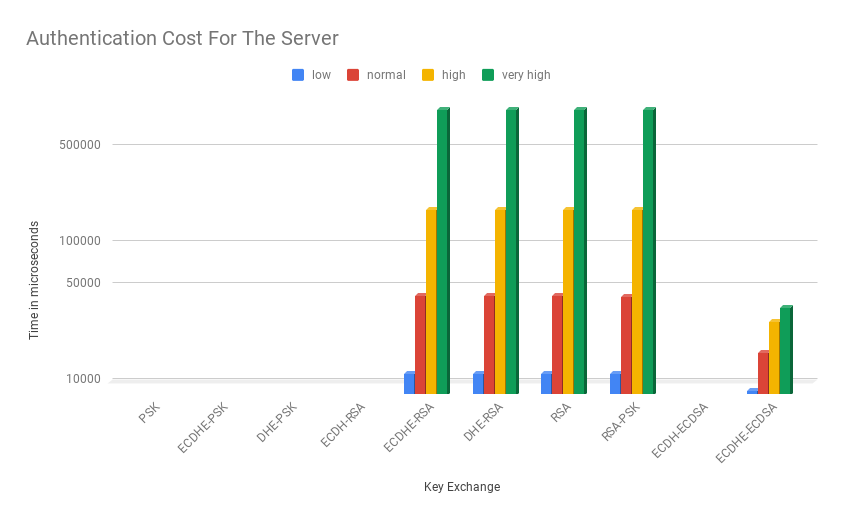
\includegraphics[width=1.0\textwidth]{img/papi-server-auth-cost.png}
					\centering \caption{Authentication cost for the server in microseconds (logarithmic scale)}
					\label{af:2}
				  \end{figure}
  
				  \begin{figure}
					\centering
					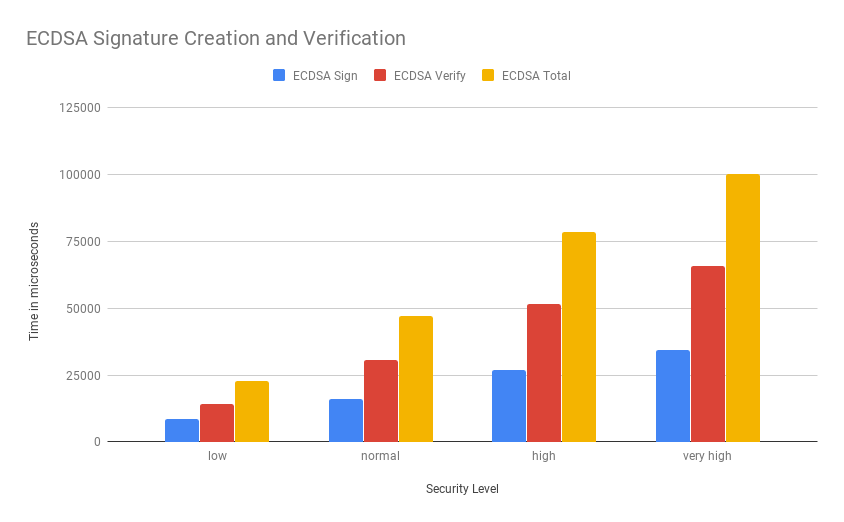
\includegraphics[width=1.0\textwidth]{img/papi-ecdsa-sign-verify.png}
					\centering \caption{ECDSA signature creation and verification costs in microseconds}
					\label{af:3}
				  \end{figure}
  
				  \begin{figure}
					\centering
					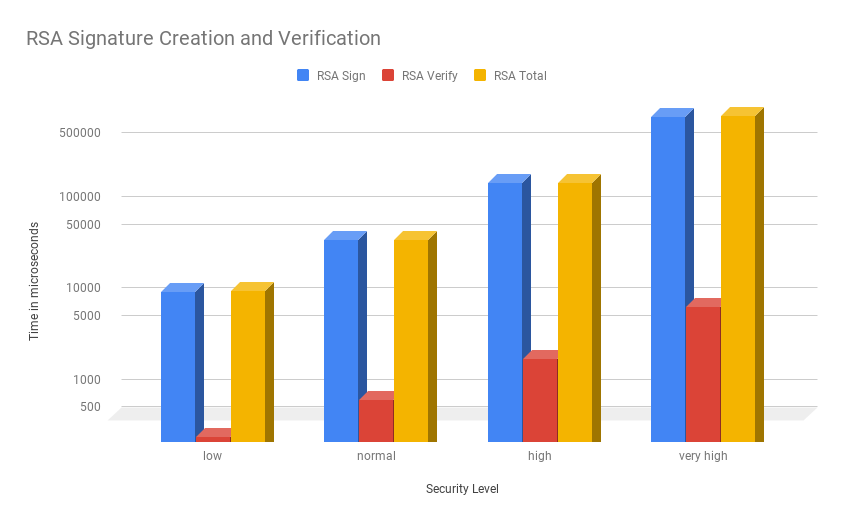
\includegraphics[width=1.0\textwidth]{img/papi-rsa-sign-verify.png}
					\centering \caption{RSA signature creation and verification costs in microseconds (logarithmic scale)}
					\label{af:4}
				  \end{figure}
  
				  \begin{figure}
					\centering
					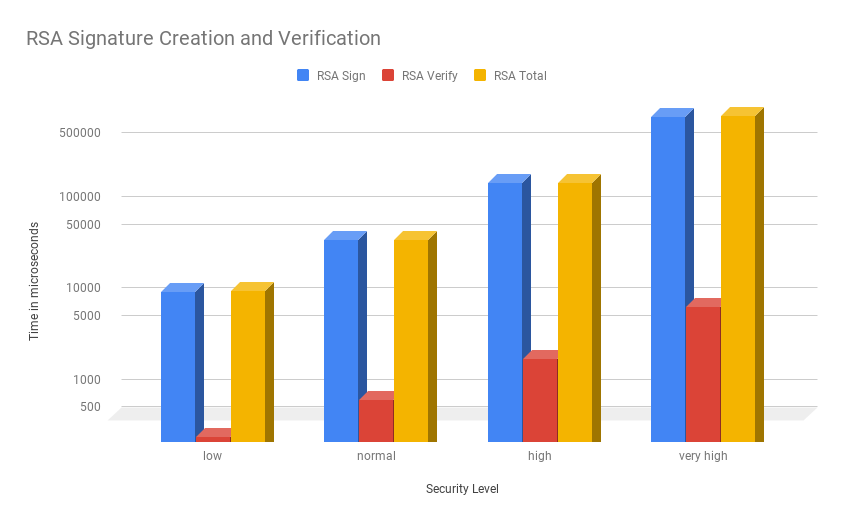
\includegraphics[width=1.0\textwidth]{img/papi-rsa-sign-verify.png}
					\centering \caption{RSA encryption and decryption costs in microseconds (logarithmic scale)}
					\label{af:5}
				  \end{figure}
  
				  \begin{figure}
					\centering
					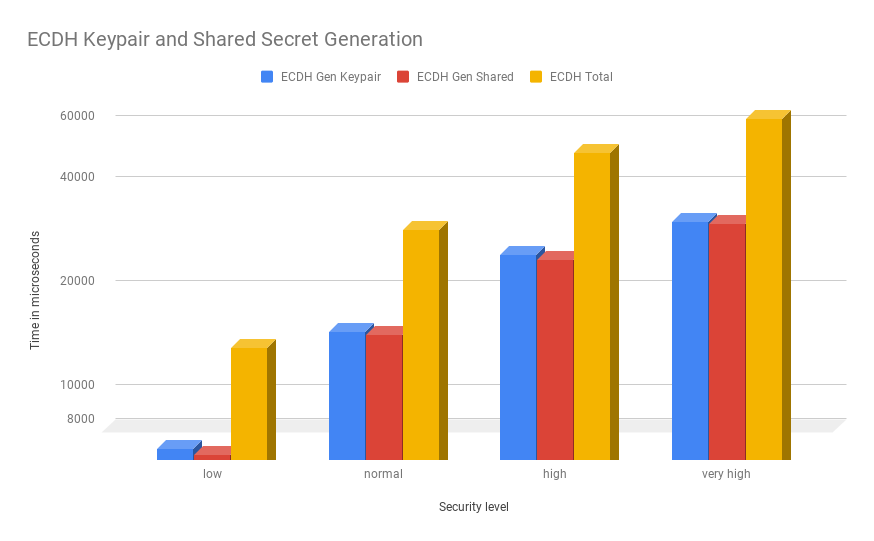
\includegraphics[width=1.0\textwidth]{img/papi-ecdh-cost.png}
					\centering \caption{ECDH keypair and shared secret generation costs in microseconds (logarithmic scale)}
					\label{af:6}
				  \end{figure}
  
				  \begin{figure}
					\centering
					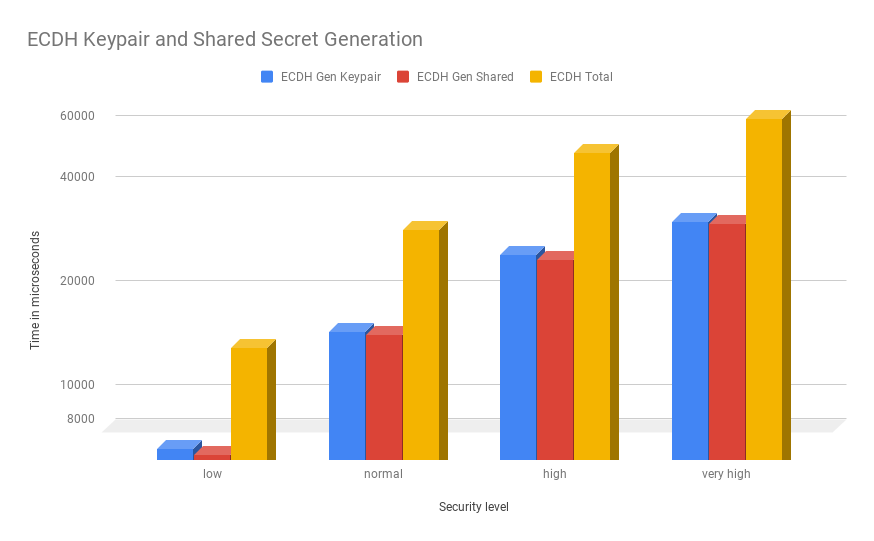
\includegraphics[width=1.0\textwidth]{img/papi-ecdh-cost.png}
					\centering \caption{DH keypair and shared secret generation costs in microseconds (logarithmic scale)}
					\label{af:7}
				  \end{figure}
   % file "Thesis_Appendix_A.tex"
\cleardoublepage

% re-set arabic numbering (B.1,B.2,...) (optional, use only if chapter prefix is added)
%\setcounter{page}{1}

%%%%%%%%%%%%%%%%%%%%%%%%%%%%%%%%%%%%%%%%%%%%%%%%%%%%%%%%%%%%%%%%%%%%%%%%%
%                                                                      %
%     File: Thesis_Appendix_B.tex                                      %
%     Tex Master: Thesis.tex                                           %
%                                                                      %
%     Author: Andre C. Marta                                           %
%     Last modified :  2 Jul 2015                                      %
%                                                                      %
%%%%%%%%%%%%%%%%%%%%%%%%%%%%%%%%%%%%%%%%%%%%%%%%%%%%%%%%%%%%%%%%%%%%%%%%

\chapter{Technical Datasheets}
\label{chapter:appendixDatasheets}

It is possible to add PDF files to the document, such as technical sheets of some equipment used in the work.

% ----------------------------------------------------------------------
\section{Some Datasheet}
\label{section:datasheet}

% See more options to include PDF files in
% http://mirror.unl.edu/ctan/macros/latex/contrib/pdfpages/pdfpages.pdf
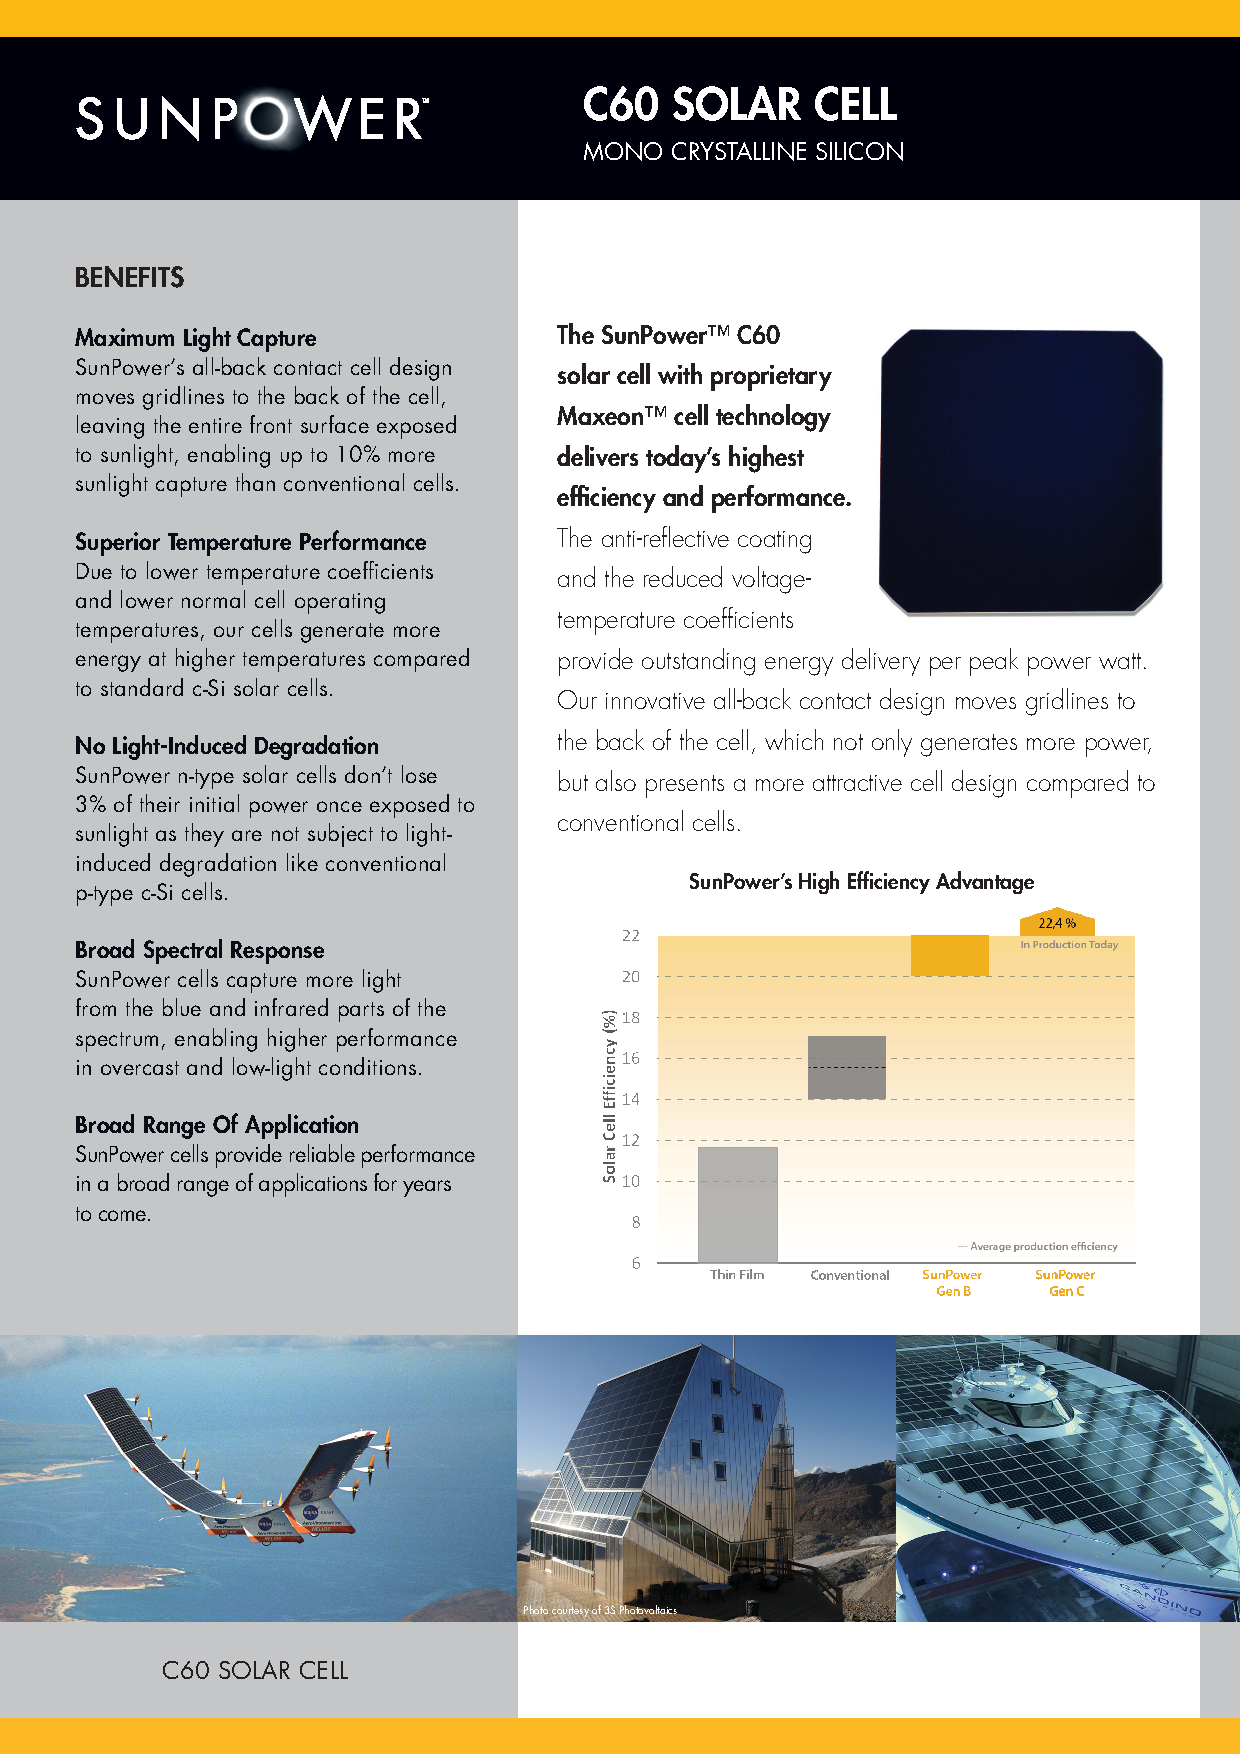
\includepdf[pages={1-2},nup=1x2,landscape=true]{Figures/SolarCell_Sunpower_C60.pdf}

 % file "Thesis_Appendix_B.tex"
%\cleardoublepage

% ----------------------------------------------------------------------
\end{document}
% ----------------------------------------------------------------------

